\documentclass[a4paper,12pt]{report}

\usepackage[spanish]{babel}

\usepackage[utf8]{inputenc}

\usepackage{setspace}

\usepackage{graphicx}

\usepackage{titlesec}
 
\titleformat{\chapter}[display]
  {\normalfont\bfseries}{}{0pt}{\Huge}
  
\pagestyle{plain}

\doublespacing

\author{
  Fernando Garcia Corona\\
  \texttt{https://github.com/FerCorona/crown}
}
\title{DESARROLLO DE UNA LIBRERÍA NPM DE FRONT-END BASADA EN COMPONENTES DE REACT PARA EL ÁGIL MAQUETADO DE UNA PÁGINA WEB USANDO BUENAS PRÁCTICAS DE DISEÑO UX/UI}


\begin{document}
	\maketitle

	\tableofcontents
	
		\chapter {INTRODUCCIÓN}
			
		\chapter {JUSTIFICACIÓN }
			Actualmente, el desarrollo de páginas Web es una de las oportunidades de empleo con mayor demanda dentro del área de la informática, en los principales buscadores de empleo  \cite{work} se pueden encontrar una área de oportunidad para ejercer. El desarrollo Front-End, de páginas Web, es una de las subáreas más buscadas por las empresas que implementan servicios basados en Web, o que de alguna manera consumen algún producto. 
El famoso sitio Stackoverflow  \cite{stackOverflow}realiza una serie de estadísticas anuales en las cuales da a conocer los lenguajes de programación en los cuales ellos obtienen un mayor número de búsquedas y respuestas. Las estadísticas muestran que, durante el transcurso del año pasado (2020), el lenguaje más usado por la comunidad de desarrolladores profesionales es Javascript. 
Por otra parte, dentro esta serie de estadísticas se cuenta con un apartado para los marcos de trabajo, en el cual encontramos que en segundo puesto está React, solo por debajo de jQuery el cual puede ser empotrado dentro de React.  Finalmente se encontró que la biblioteca número uno es Node.js. 
El desarrollo Front-End  \cite{frontEnd}de páginas Web consiste en hacer la visualización que tenemos cuando ingresamos a algún sitio desde nuestro navegador, para esto es necesario que el programador que realiza la tarea tenga conocimientos básicos de HTML, CSS y JavaScript, para que sea posible construir una Web sencilla. Cabe destacar que un desarrollador Front-End no es el encargado de diseñar la experiencia de usuario ni tampoco el diseño de interfaz gráfica, ya que para esto existen otras disciplinas especializadas, pero en caso de tener conocimiento en el área puede agregar una herramienta que puede combinarse y agregar habilidades.
\newline
En la medida que una Web escala, esta tiende a aumentar su complejidad de desarrollo si no se comienzan a usar bibliotecas o marco de trabajos, que nos permiten a tener un trabajo más limpio, organizado, seguro y modulable. 
Como se mencionó anteriormente Javascript es usado tanto de manera profesional como con otros fines como los académicos, este lenguaje cuenta con un gestor de paquetes denominado NPM  \cite{npm},  que permite que se agreguen miles de funcionalidades extras a tu proyecto, NPM consiste en un cliente de líneas de comandos con el cual es posible agregar a nuestro proyecto paquetes, estos paquetes son de utilidad porque podemos reusar código que alguien más ya desarrollo, probó y decidió compartirlo, haciendo que el trabajo sea más ágil.  De igual manera nosotros podemos aportar publicando nuestra biblioteca. Dentro de NPM contamos con miles de bibliotecas de código abierto.  
Teniendo esto en cuenta, nos da la posibilidad de tener nuestra propia biblioteca y publicarla, para que personas a las cuales tienen alguna necesidad, pero no cuentan con el tiempo de ejecutarla puedan acceder a la nuestra, e incluso nosotros mismos usarlas en posteriores proyectos. 

El desarrollo de software de código abierto \cite{openSource} consiste en publicar algún tipo de herramienta propia, el cual será de licencia pública para que más personas puedan acceder al código fuente, si lo desean podrán usarlo o adecuarlo a sus necesidades. 
Anteriormente se mencionó un marco de trabajo de Front-End llamado React, este es mantenido por Facebook desde mayo del 2013 que fue su fecha de publicación, en la actualidad tiene más de mil contribuidores según lo indica el repositorio oficial. 
Algunas de las particularidades de React  \cite{reactOreilly}es que nos motiva a crear componentes que pueden ser utilizados más veces, y de esta manera tener una menor cantidad de código y más reutilizable. 
Nos deja crear una aplicación en una sola página que de ser de una manera tradicional y a gran escala se convertirían en una tarea imposible.
\newline
Por el uso desmedido de cada una de las tecnologías que se han mencionado nace la razón por la cual se desea desarrollar una biblioteca de NPM, la cual ayudará grandemente a la comunidad de desarrolladores de páginas Web y esto principalmente a las personas que cubren el rol de programadores Front-End. 
Esta biblioteca permitiría a los desarrolladores agilizar su carga de trabajo, poniendo a su alcance un conjunto de elementos usados en el desarrollo Front-End, alguno de ellos son botones, textos, etiquetas de texto, tablas, checkbox, radio botones, etc.  Los cuáles serán elementos definidos, que contarán con una definición de estilos \cite{scss} (CSS) establecidos, cada componente permitirá al desarrollador modificar parámetros básicos como el color, el texto y acción que va a realizar, esto con el fin de adaptarlo a las necesidades propias del proyecto en el que se va a hacer la implementación de la biblioteca.  
Otra ventaja por parte de la biblioteca es que esta estará basada en prácticas modernas del diseño UI/UX, como lo es Mobile First \cite{mobileFirst} Indexing (ideología de Google), que nos pide enfocar el diseño de cualquier Web primero para dispositivos móviles, ya que afirman que es en el mercado el cual consume más contenido Web, ayudándonos a no requerir un conocimiento avanzado sobre el diseño de interfaces gráficas. 
Esto nos dará la garantía de la experiencia del usuario, lo que significa que el usuario sabrá que está haciendo en todo momento, y también estaremos otorgando un diseño de interfaz moderno.
Ya que el diseño de cada elemento de la biblioteca estará diseñado para ser fácil de usar para el desarrollador y usuario final y garantizar que el resultado del desarrollador sea el mejor para el usuario final.
Finalmente, además de los elementos básicos que incluirá la biblioteca, tendrá más elementos que permitirán aún más la eficiencia, contendrá otros elementos compuestos como formularios, tarjetas, alertas, pies de página, menús de navegación, elementos deslizables. 

La última parte de la biblioteca consistirá en elementos aún más compuestos, denominados plantillas que consiste en pantallas de login, registro, página de inicio entre otras. Abriendo la posibilidad que más personas puedan aportar creando sus propias plantillas, y crear una comunidad de desarrollo.  
Debemos tomar en cuenta que este proyecto no se puede clasificar dentro del área de los marco de trabajos ya que para ser parte de, es necesario contemplar toda la estructura necesaria dentro de una página Web, modelos, vistas y controladores (MVC). Nuestro proyecto está focalizado en las vistas, por lo cual puede clasificarse como biblioteca.  
  
Con el uso de esta biblioteca reduciremos el tiempo de desarrollo, ya que no comenzaremos a escribir HTML y  CSS desde cero, tendremos una base común sobre la cual podemos seguir. Todo el equipo tendrá los mismos estilos y evitaremos que nuestra Web tenga discrepancias dentro de los diferentes módulos o vistas que tiene nuestra Web. 
Al usar esta biblioteca nos aseguraremos de que las vistas de nuestra aplicación Web puedan mirarse estéticamente iguales y tendemos la seguridad de que luzca de la misma forma en Chrome, Safari Firefox o un mayor número de navegadores, no importa si es una versión actual o una más antigua. 
Con esta biblioteca evitamos el tiempo de aprender un nuevo marco de trabajo, ya que funciona sobre React y los conocimientos necesarios son saber React. 
Tendríamos una organización predeterminada para todo el proyecto en el que se implementa, teniendo uniformidad en el desarrollo y en la interfaz gráfica, aumentando la agilidad en el trabajo y de manera proporcional reduciendo el tiempo y primordialmente el costo que implica, también reducirá el mantenimiento, así como los posibles errores. 
Debemos tomar en cuenta que el número de personas que participan en el desarrollo de un software es variado, pero regularmente este es mayor a uno, por lo que es conveniente que el código sea claro, legible y reutilizable para que el mayor número de personas que están involucradas, para que puedan trabajar en la mayor parte del proyecto sin problemas en caso de que exista un cambio de roles, es por lo que usar una biblioteca estandariza el trabajo. 
Las bibliotecas cumplen con gran cantidad de pruebas, para que no surjan problemas y sean impedimento al implementarlas, esta no será la excepción al incluir pruebas de validación, así también se eliminan errores en el proyecto donde se implementan. 
  
Lamentablemente como en todo marco de trabajo y biblioteca existe la desventaja a que al implementarlo este te fuerza a verte limitado con respecto a la cantidad de configuración y personalización que podemos editar \cite{newTech}. Otra cosa por tomar en cuenta es que no se necesita aprender una sintaxis específica para usar esta biblioteca, pero es necesario conocer la sintaxis que se usa con React, ya que esta biblioteca es basada en React, y es necesario conocer los conceptos básicos como el uso de componentes y el paso de elemento. Al usar una nueva biblioteca es posible que sientas que estás perdiendo el tiempo al incorporarlo en proyectos, debido al tiempo de aprendizaje. También no se encuentra recomendable agregar la biblioteca en un proyecto que ya está avanzado, y no lo es por el funcionamiento o incompatibilidad de bibliotecas, esto es más bien, porque no es viable visualmente ya que se encontrara elementos y vistas distintas unas entre otras, esto, si no se decide actualizar los elementos existentes lo cual aumenta el tiempo de desarrollo.


Debemos considerar que al agregar una capa software extra a nuestro Proyecto aumenta en tamaño, ya que además del peso de React que es necesaria para usar esta biblioteca debemos contar el peso de nuestra biblioteca en sí, aunque no todas  las tecnologías  mencionadas son agregadas en la versión que estará alojado en el proyecto, ya que por ejemplo Webpack \cite{webPack}, solo es usado durante el desarrollo.

Al usar la presente biblioteca se acorta el trabajo necesario, que es requerido después de que el maquetado de nuestra página Web está listo, ya que a diferencia de otras bibliotecas  como Material Design solo se enfocan el maquetado pero esta biblioteca se involucra en la funcionalidad de los componentes.

Una vez un componente de esta biblioteca, se implemente,  este no necesitará trabajo extra, el componente estará listo para ser utilizado, por ejemplo para el componente de entrada de texto estará directamente conectado con el estado de React, eso significa que cuando necesitemos el dato introducido ya lo tendremos listo, y no como en React simple que debemos procesar el input para poder obtener el dato.

Esto deja la biblioteca como una opción híbrida entre el maquetado simple conformado por HTML, CSS etc. y el procesamiento de los datos con JavaScript y PHP.

\newpage
		
		\chapter {OBJETIVOS }
			\section {OBJETIVOS GENERALES}
				Desarrollar una librería para el desarrollo de páginas Web, especialmente para el área de front-end, publicada en el gestor de paquetes de JavaScript “NPM”, usando el framework React, permitiéndonos la utilización de componentes para facilitar, agilizar y mejorar el maquetado de una página Web, incluyendo prácticas de diseño UI/UX que permiten que el usuario llegue a entender el funcionamiento de la aplicación sin que se requiera un entrenamiento de la misma, haciendo el sito que implemente la librería fácil de usar y atractiva visualmente. 

			
			\section {OBJETIVOS ESPECÍFICOS} 
				  \begin{itemize}
 \item Desarrollar una librería para el desarrollo Front-End de páginas Web.
 \item Publicar la biblioteca para su uso con el gestor de paquetes de JavaScript \cite{javascript} llamado NPM.
 \item Usar el marco de referencia React que nos permite la creación de componentes reutilizables.
 \item Implementar Web-pack para garantizar el funcionamiento de la biblioteca ya que nos permite empaquetar y exportar todos los módulos y dependencias que incluye nuestra librería en un solo archivo para la correcta y ágil implementación. 
 \item Aunado a esto se utilizará Babel \cite{babel} que es un convertidor de código JavaScript a versiones anteriores, lo que nos permitirá una gran cantidad de compatibilidad con navegadores antiguos. 
 \item Para unificar nuestra sintaxis se usará ESLint el cual nos permite definir una guía de estilos para la librería, sobre esto se usará una guía de estilos ya definida y probada, la de Airbnb. 
   \end{itemize}
\newpage

			
		\chapter {ALCANCES Y LIMITACIONES }
		
		\chapter {MARCO TEÓRICO  }
			    \begin{itemize}
    
    	\item \textbf{Librería Front-end:} Una librería Front-end \cite{frontEnd2}es una herramienta que es agregada a nuestros proyectos, en este caso web, el cual incorpora elementos que otras personas o equipos ya desarrollaron, sumando funcionalidad a nuestra web, reduce el mantenimiento y el tiempo de desarrollo, algunas características que existen actualmente y pueden agregarse van desde gráficas, animaciones, mapas etc. 
      
       \item \textbf{NPM :} NPM \cite{npm} es un gestor de paquetes que nos permite agregar dependencias a cualquier proyecto basado en Javascript, esto es posible con un cliente de líneas de comandos que es útil para poner o quitar los paquetes que deseamos. La configuración consta de un archivo en el cual contiene una lista de las dependencias que se quieren instalar en nuestro proyecto. Actualmente existen miles de paquetes que pueden ser descargados de manera gratuita y de igual manera permite colaborar. 
       
       \item \textbf{ React :} React \cite{react} es una librería de Javascript para el desarrollo de interfaces de usuario (Front-end), famosa por la posibilidad de hacer fácilmente webs de usa sola página. React fue desarrollada por Facebook y con el paso del tiempo, conocidas empresas han empezado a implementarlo en sus proyectos. 
    React nos permite desarrollar de una forma más ordenada y con el menos código necesario. 
    Se considera que React no es un Framework en comparación con ANGULAR o EMBER porque no tiene cada una de las áreas que propone el modelo vista controlador, este solo se encarga de las vistas. 
    Uno de los puntos fuertes de React es que cuenta con un DOM virtual el cual es almacenado en memoria, esto provoca que cuando algo cambie este se va reflejado en memoria de una forma más rápida, después el DOM virtual será comparado con el DOM del navegador y solo actualizara lo que encuentre diferente. 
    React funciona en base a componentes que pueden ser reusados cuantas veces sea necesario, una forma fácil de entenderlo puede ser como la programación orientada a objetos al hacer una instancia de una clase, estos componentes pueden tener un estado, que es encapsulado por sí solo, de manera local por cada uno y puede ser actualizado.  
    
       \item \textbf{HTML  :}   HTML \cite{html} es un lenguaje con un conjunto de etiquetas que permite definir el contenido con el que podemos interactuar dentro de una página web. 
       
       \item \textbf{ SASS :} SASS \cite{scss} es un preprocesador de CSS, el cual nos ayuda a agregar características que no tiene CSS puro y que son propias de los lenguajes de programación como variables, funciones, herencia entre otros. Nos permite dedicar menos tiempo para mantener y crear el CSS y agrega la posibilidad de tener una organización modular. 
       
       \item \textbf{ Webpack :} Hace algunos años Javascript iniciaba como un lenguaje que nos permitía agregar interacción a nuestras páginas web, que anteriormente eran simplemente contenido estático.  Javascript nos permitía recuperar los datos que eran introducidos en formularios, podíamos mostrar ventanas emergentes o incluso agregar animaciones. Para agregar Javascript en nuestros archivos de HTML, se debía agregar la etiqueta <script>, donde se indicaba la ruta donde estaba almacenado nuestro archivo .js de Javascript.  
    Años más tarde se agregó soporte al lenguaje Javascript, para permitir hacer peticiones asíncronas a nuestros servidores, esto hizo que las empresas empezaran a ver como viable el desarrollo web, que previamente estaba enfocado en el desarrollo de escritorio, también hizo que los archivos .js empezaran a crecer en cantidad de líneas en nuestros proyectos, y se miraba reflejado en nuestros archivos .html los cuales empezaron a tener múltiples etiquetas <script>. Lo que significaba múltiples peticiones para obtener los archivos del servidor, esto agregaba una capa de complejidad, debido a la inclusión de múltiples archivos .js embebidos en un .html y al agregarlos se debe tener en cuenta el orden en que se listan, porque es posible que tengan dependencias entre ellos. Actualmente es posible comprimir los múltiples archivos .js para que sean menos peticiones al servidor (CDN).  Cuando un proyecto con Javascript crecía aumentaba el número de módulos que se agregan, pero no existía la forma de gestionarlos. Un problema que tenía Javascript es que los navegadores no soportan un sistema nativo de módulos por eso se agregaron Require.js y Common JS. 
    En base a esto nació Webpack \cite{webPack} que permite usar NPM como gestor de dependencias y soporta el sistema de módulos Common JS.
    Webpack permite modular nuestro código, para esto genera un grafo dado un punto de entrada, el punto de entrada es el nodo inicial de nuestro grafo, el grafo es generado con las inclusiones de elementos encontrados en los archivos, como son imágenes, archivos de CSS etc. Esto genera un archivo final en el que estará el empaquetado de nuestros archivos. 
    Webpack nos permite especificar cargadores para distintos tipos de archivos como imágenes, SCSS, CSS, HTML. JSX, etc. ya que nativamente solo admite archivos Javascript. 
    La configuración es dada por un archivo que se coloca en la raíz del proyecto.
    
       \item \textbf{Babel  :}   Babel \cite{babel} es un traductor de código Javascript, que permite convertir el código Javascript más moderno en alguna versión más vieja, esto nos proporcionó la capacidad de que nuestro código pueda ser ejecutado por más cantidad de navegadores, los cuales solo pueden interpretar versiones anteriores de Javascript. Por ejemplo, el siguiente código es usado en React para mostrar un texto. 
    \begin{figure}[H]
    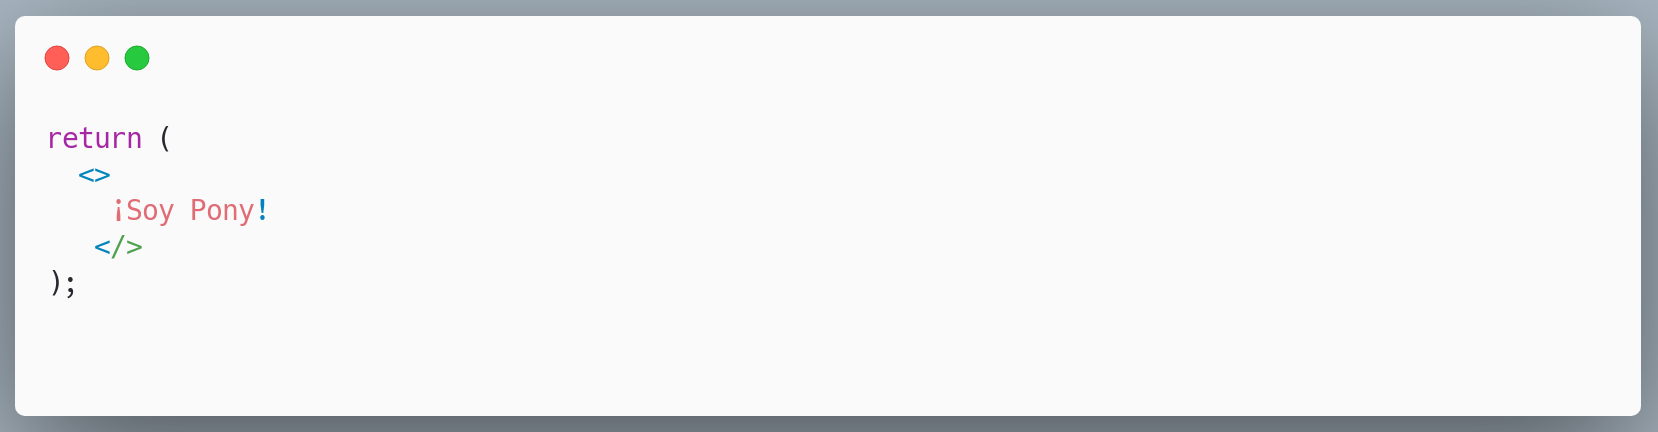
\includegraphics[width=1\textwidth]{./Imagenes/image16.png}
    \caption[Impresión de texto con React]{Impresión de texto con React}
    \end{figure}
       El código será convertido en el que se muestra En la figura 7.2, el cual es interpretada por un mayor número de navegadores. 
       \newline
       \newline
       \begin{figure}[H]
       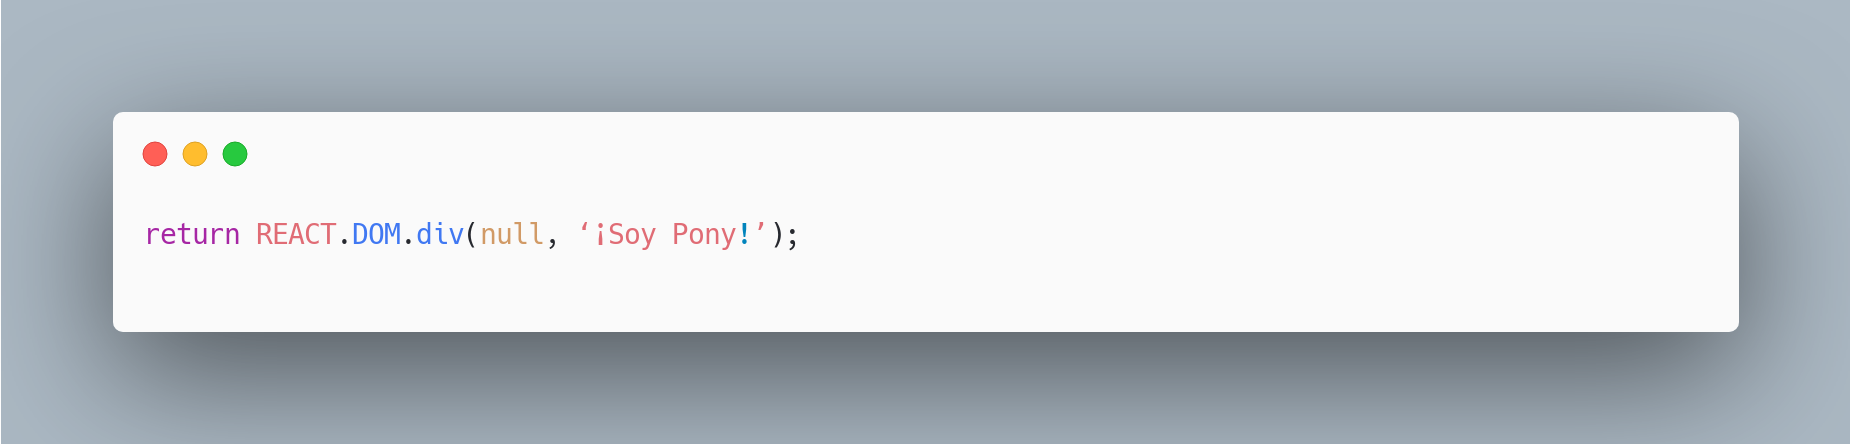
\includegraphics[width=1\textwidth]{./Imagenes/image5.png}
        \caption[Impresión de texto una vez el código es convertido]{Impresión de texto una vez el código es convertido}
       \end{figure}
       \newline
       \newline
       \item \textbf{ESLint :}ESLint nos permite definir una guía de estilos en nuestro código, lo que nos ayudará a tener un código limpio y claro para que sea fácil de editar y mantener, podemos agregar guías de estilos una de ellas es la de Airbnb, que es una de las más usadas. 
       
    \end{itemize}
		
		\chapter {PROCEDIMIENTO Y DESCRIPCIÓN DE LAS ACTIVIDADES REALIZADAS}
			        El objetivo de desarrollo de la presente librería se basa en el siguiente principio, “ cuando un elemento sea actualizado, sea un botón, cuadro de estado, entrada de texto, etc. el componente regresará un objeto el cual tendrá el nombre del elemento y el nuevo valor para que este sea actualizado en el state de React ”.  Con esto deseamos generar el  flujo de la Figura 8.1.
        
               \begin{figure}[H]
           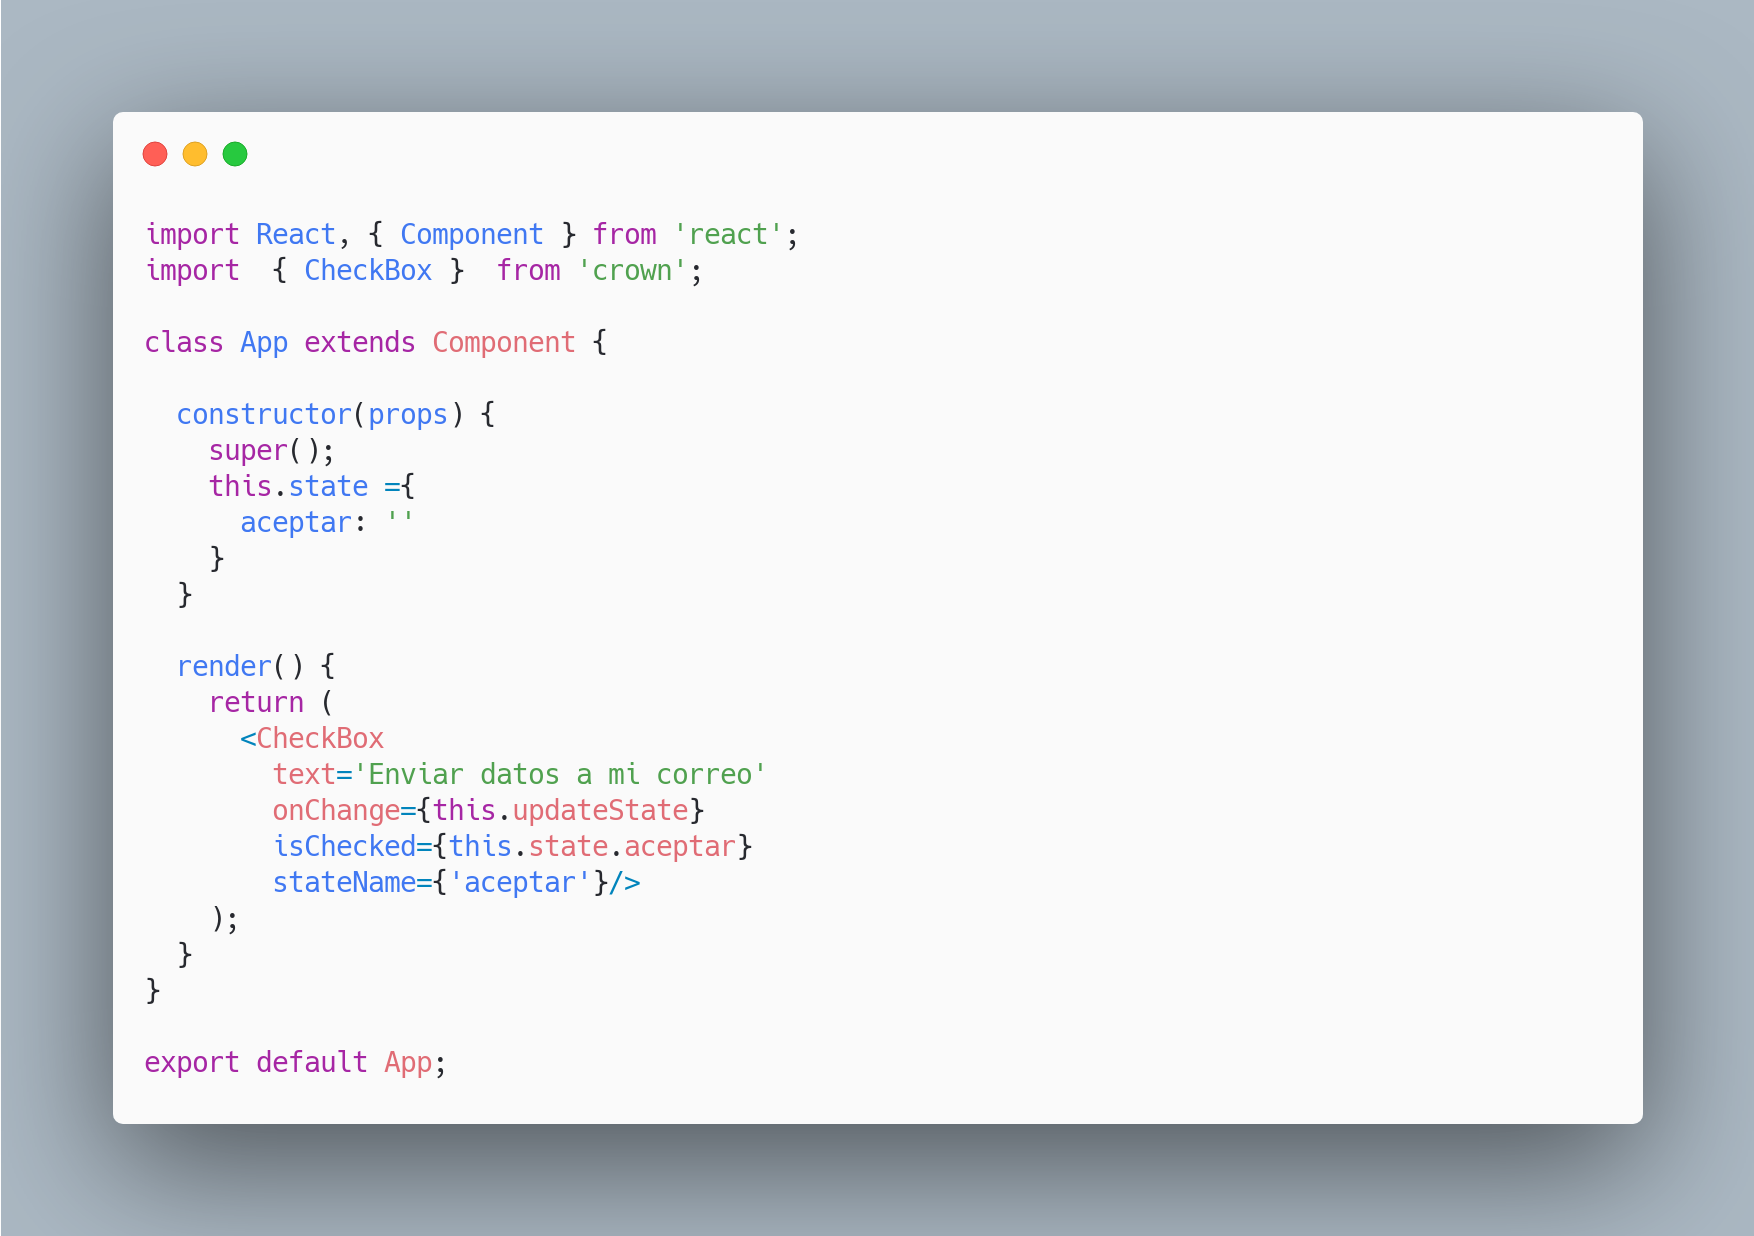
\includegraphics[width=1\textwidth]{./Imagenes/carbon-8.png}
           \caption[Resultado esperado de la librería]{Resultado esperado de la librería}
             \end{figure}
        
        Importamos el elemento CheckBox desde “crown” dentro de el método render en return  ponemos el componente CheckBox y le damos los  siguientes  props.
        
        \begin{itemize}
        	\item \textbf{onChange:} Función que actualiza el estado, que definiremos adelante.
        	\item \textbf{isChecked::} Ponemos el valor de “aceptar” que está en el estado.
        	\item \textbf{stateName:}  Es el nombre ( y no el valor como en isChecked ) con el que identificamos el elemento en el estado. 
        \end{itemize}
        
        \newline
        Dentro del componente CheckBox se devuelve un objeto como el que se muestra en seguida.
        \begin{figure}[H]
         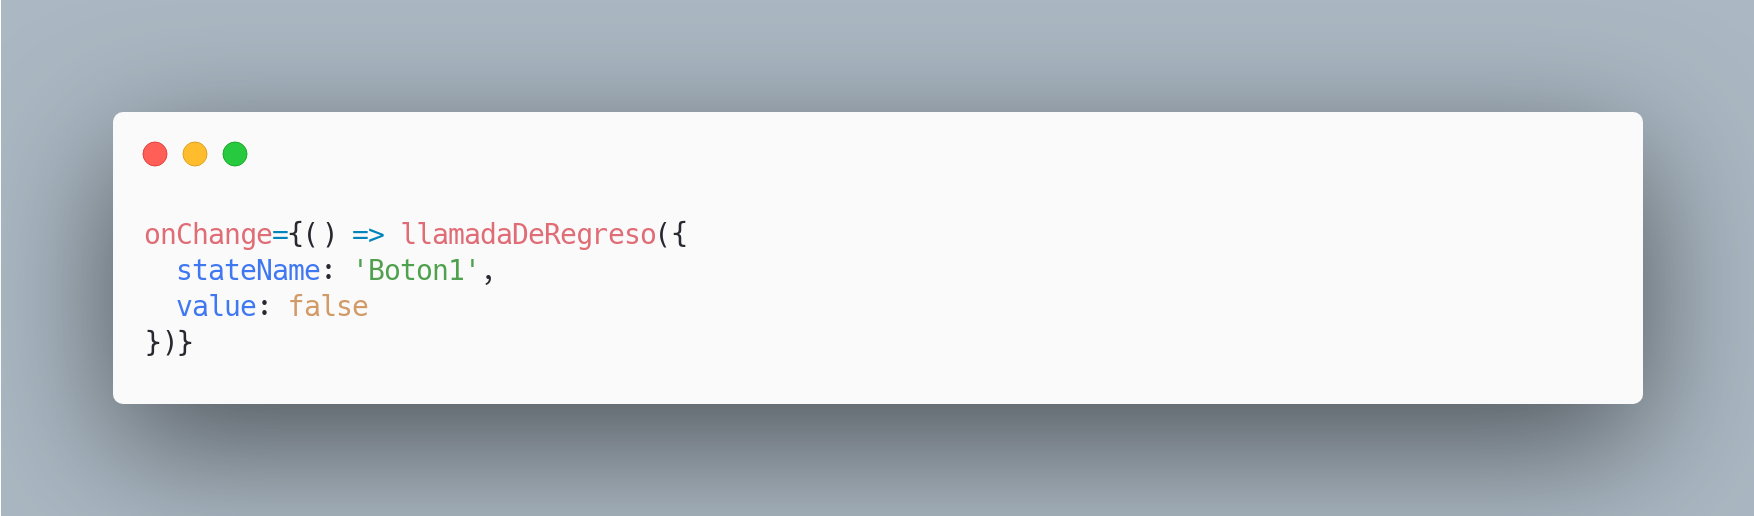
\includegraphics[width=1\textwidth]{./Imagenes/carbon-6.png}
         \caption[Resultado de la llamada]{Resultado de la llamada}
             \end{figure}
        \begin{itemize}
        	\item \textbf{onChange:}  Este es el evento que se ejecuta cuando una acción es disparada, por ejemplo cuando haces click en un CheckBox.
        	\item \textbf{llamadaDeRegreso:} Es la función que recibe el componente, y cuando se hace click en un CheckBox este, por defecto llama la acción que está dentro del evento onChange. En este caso llama a llamadaDeRegreso.
        	\item \textbf{stateName:}  Es el nombre ( y no el valor como en isChecked ) con el que identificamos el elemento en el estado. 
        	\item \textbf{value:}  Este dato almacena el valor actualizado del elemento, esto define si el CheckBox está seleccionado o no.
        \end{itemize}
        \newline
        Esto facilitará a tener una única función ( Figura 8.3 ) capaz de actualizar todos los elemento que agregamos ya que contamos con el nombre,  que es con el que se identifica en el estado y también el nuevo valor.
        \begin{figure}[H]
         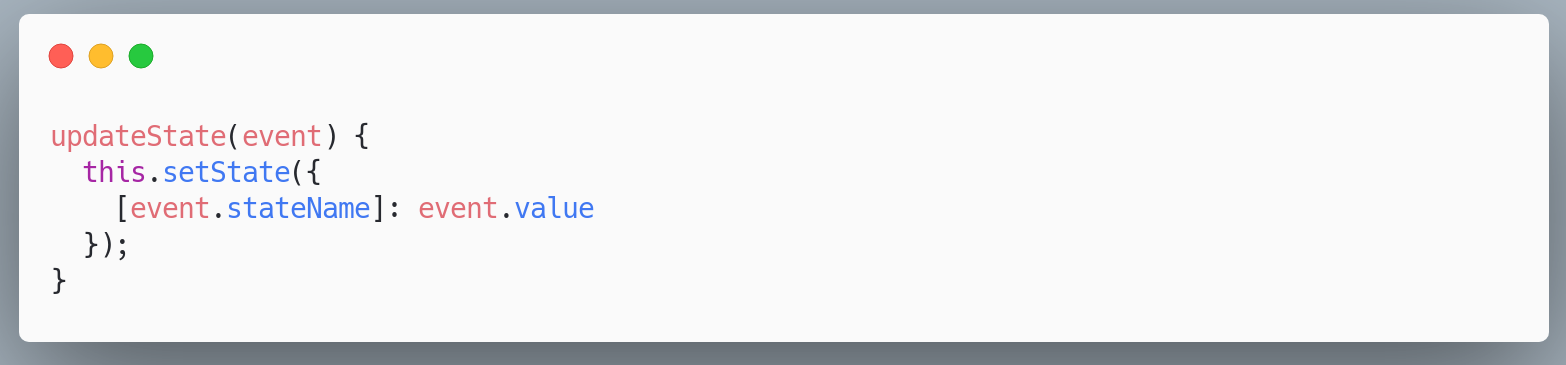
\includegraphics[width=1\textwidth]{./Imagenes/carbon-7.png}
         \caption[Actualización del estado]{Actualización del estado}
             \end{figure}
        \newline
        
        \end{enumerate}
			
			\section {CREACIÓN DEL AMBIENTE DE DESARROLLO}
				    \subsection{Ambiente De Desarrollo}
    Durante el desarrollo de la presente librería se usó el sistema operativo MacOS, con la terminal que se incorpora por defecto en el mismo.
    El primer paso que se debe realizarse es colocarse en el directorio en el que se desea trabajar, esta librería se sitúa en la carpeta Documentos durante el desarrollo, usando el comando de la Figura 8.4 es posible cambiar de directorio, ejecutandolo en la terminal.
    
    \newline
     \begin{figure}[H]
     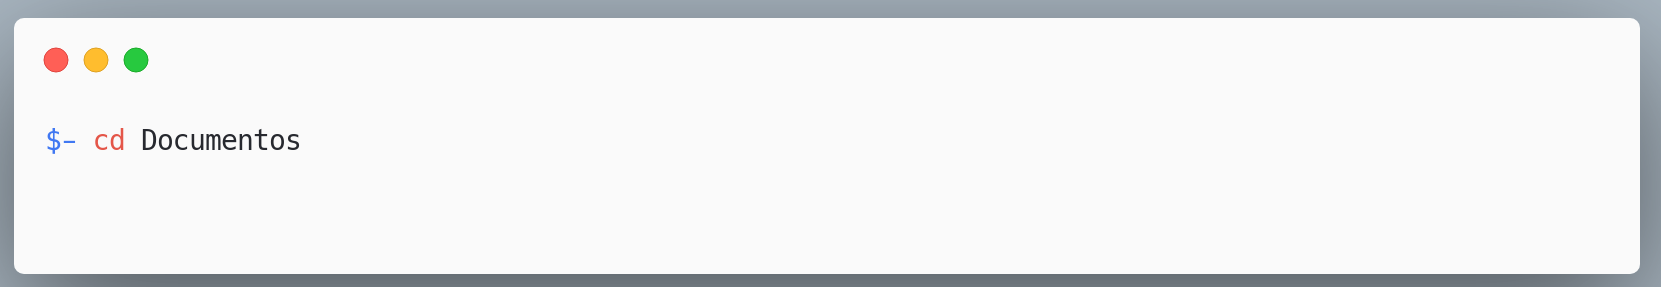
\includegraphics[width=1\textwidth]{./Imagenes/image15.png}
     \caption[Moverse entre directorios]{Moverse entre directorios}
         \end{figure}
Después se creó la carpeta de desarrollo son el siguente comando. Se llamó de manera simbólica como “crown”, que significa en español “corona”.
     \begin{figure}[H]
    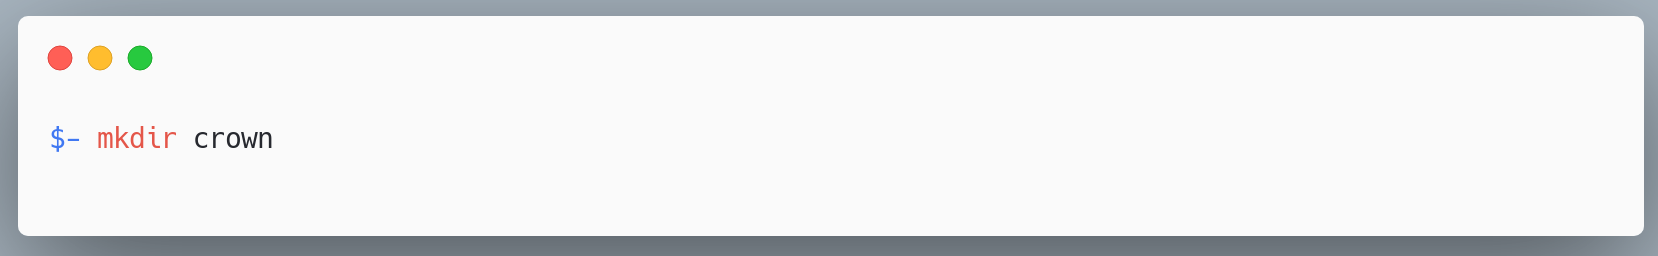
\includegraphics[width=1\textwidth]{./Imagenes/image7.png}
     \caption[Crear nuevo directorio]{Crear nuevo directorio}
         \end{figure}
    
    Dentro de esta carpeta debemos crear dos carpetas, una tendrá el código fuente, y la otra tendrá el resultado del código procesado que se importará por otros proyectos, con la ayuda del siguiente comando.
    \newline
     \begin{figure}[hbt!]
    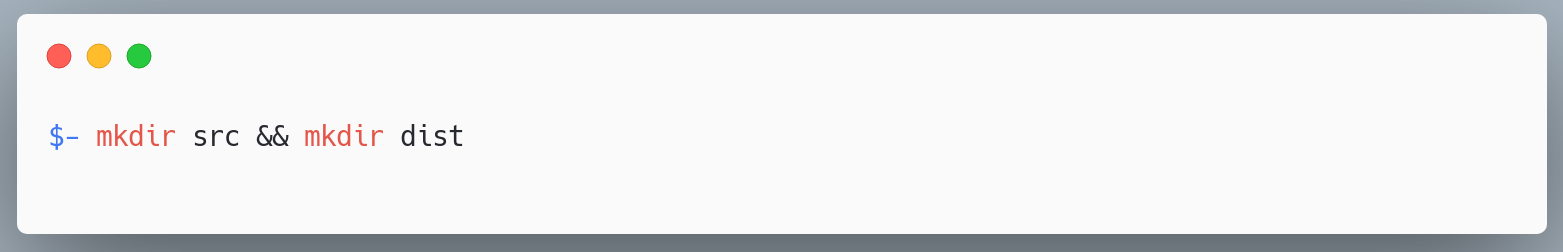
\includegraphics[width=1\textwidth]{./Imagenes/image37.png}
     \caption[Crear nuevos directorios]{Crear nuevos directorios}
         \end{figure}
    \newline
    \newline
    
    \subsection{Inicialización Del Archivo NPM}
    Se continúo inicializando el archivo de NPM, el cual nos sirve para llevar el control de las dependencias de JavaScript que se vayan agregando, esto ejecutando el siguiente comando.
    \newline
    \newline
     \begin{figure}[H]
    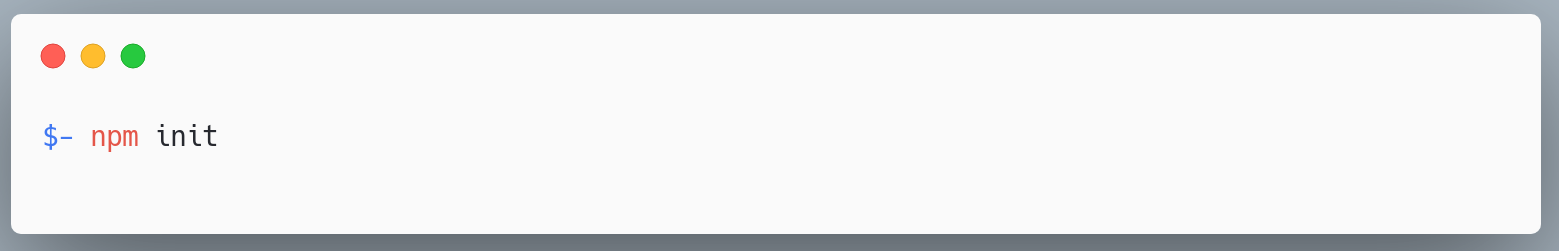
\includegraphics[width=1\textwidth]{./Imagenes/image11.png}
     \caption[Inicializar NPM]{Inicializar NPM}
         \end{figure}
    
    \newline
    \newline
    Al introducir el comando anterior este preguntara por una lista de datos necesarios, para tener el control de los paquetes, estos son los siguientes datos que se deben proporcionar:
    \begin{itemize}
    \item \textbf{Nombre del paquete:} Este es el nombre simbólico con el cual se puede identificar el paquete dentro del buscador de NPM, por lo tanto, es el nombre con el que nuestro paquete será encontrado.
    \item \textbf{Versión del paquete:}Con esta opción controlaremos la versión, y en caso de que se agreguen funcionalidades o se resuelva algún error, tendremos una manera de actualizar en los proyectos que incorporen esta librería.
    \item \textbf{Descripción del paquete: }Daremos a las personas una muy breve explicación acerca del uso que puedes obtener con nuestra librería.
    \item \textbf{Punto de entrada del paquete:} Es el directorio el cual será importado cuando agreguemos nuestra librería a otros proyectos, este podrá incluir la lógica o que solamente sea el nodo inicial de todo nuestro código.
    \item \textbf{Comando de prueba:} Dentro de este archivo nos permite incluir comandos que afectan a nuestra librería, en este caso, este comando nos sirve para ejecutar una serie de pruebas, para usar antes de publicar una nueva versión.
    \item \textbf{Repositorio de GIT del paquete:} Dentro de esta línea, debemos poner la dirección url en el cual está alojado nuestro proyecto. Este será agregado más adelante junto con el archivo de configuración de GIT.
    \item \textbf{Palabras clave del paquete:} Es una lista de palabras la cual nos ayuda para el momento cuando se inserta una búsqueda en el gestor de NPM, y pueda realizar una búsqueda basada en las palabras que describen la utilidad de nuestro paquete.
    \item \textbf{Autor del paquete:} Es el nombre del autor, autores u organización la cual está desarrollando el proyecto.
    \item \textbf{Licencia del paquete:} Existen una serie de licencias posibles a ser seleccionadas, para este caso se eligió la licencia MIT (MIT, Massachusetts Institute of Technology), que es una licencia de software que fue originada por el Instituto Tecnológico de Massachusetts, significa que el código que es producido bajo esta licencia es de uso libre, con la que damos muy pocas limitaciones de reutilización del código 
    \end{itemize}
    En la siguiente imagen se muestra un ejemplo de los datos solicitados por el comando y los datos introducidos, los cuales son de prueba y nos son los mismos que se ingresaron el proyecto original. 
    Todo esto generará un archivo final llamado package.json en el directorio raíz, este contendrá la configuración dada en este paso.
    Finalmente preguntará si la información introducida es correcta  y nos confirmara con una impresión en consola de los datos que estarán almacenados en el archivo.
    \newline
    \newline
     \begin{figure}[H]
    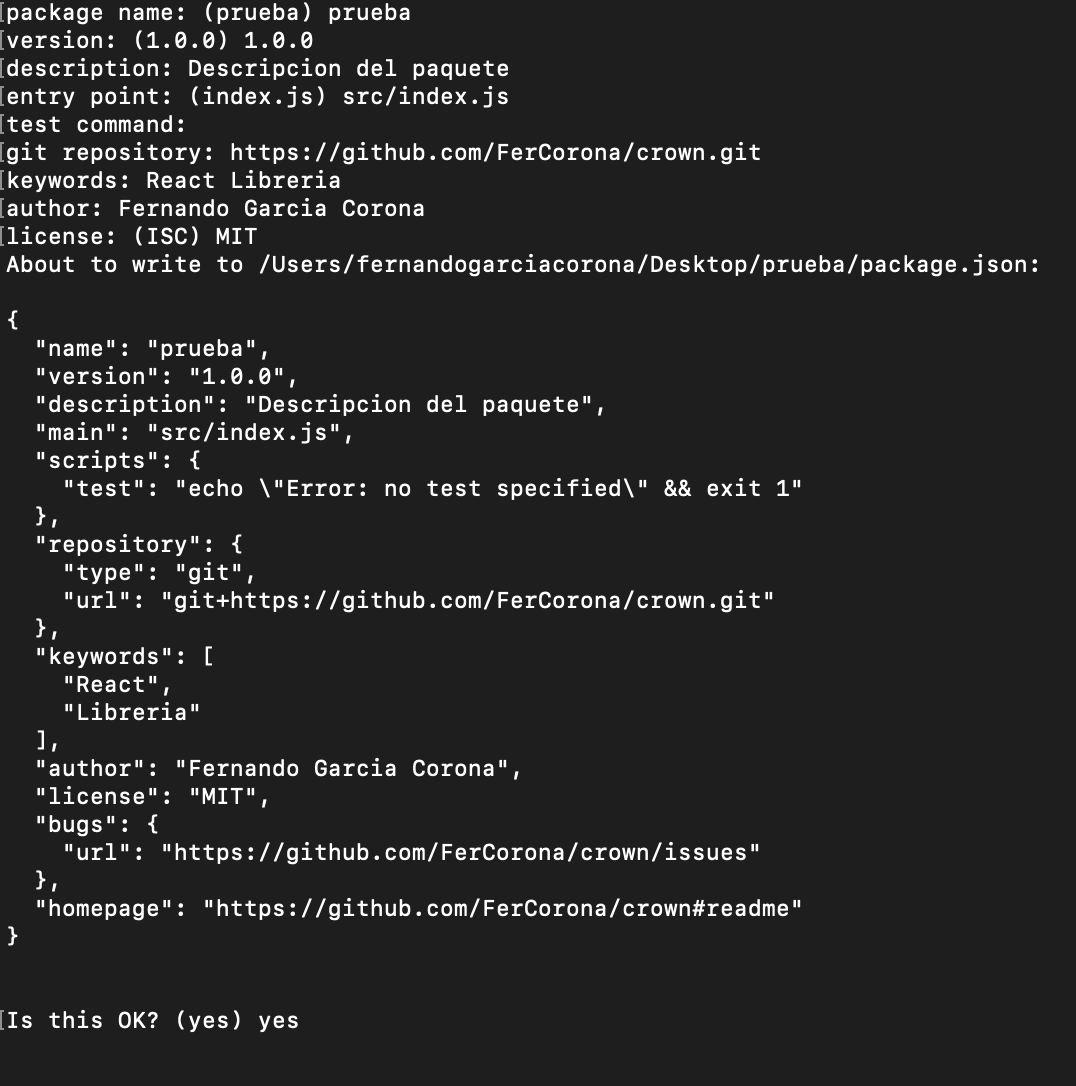
\includegraphics[width=1\textwidth]{./Imagenes/image9.png}
     \caption[Archivo de salida]{Archivo de salida}
         \end{figure}
    \newline
    \newline
    
    \subsection{Inicialización De Git En Nuestro Proyecto }
    Ahora se continuará agregando GIT en nuestro proyecto, esto nos garantizara el control de los cambios que se vayan realizando, para en caso de catástrofes poder regresar a una versión anterior, También podemos crear ramas,  para alojar nuevas funcionalidades que se requieran ser agregadas, eso sin afectar el estado del proyecto que ya está funcionando y cuando la nueva función esté completa y probada poder mezclarla con el original (la rama master).
    Incluir GIT no es una tarea compleja, basta con ejecutar el siguiente comando en la línea de comandos, esto dentro de nuestro directorio (“/Documents/crown”).
    \newline
    \newline
     \begin{figure}[H]
    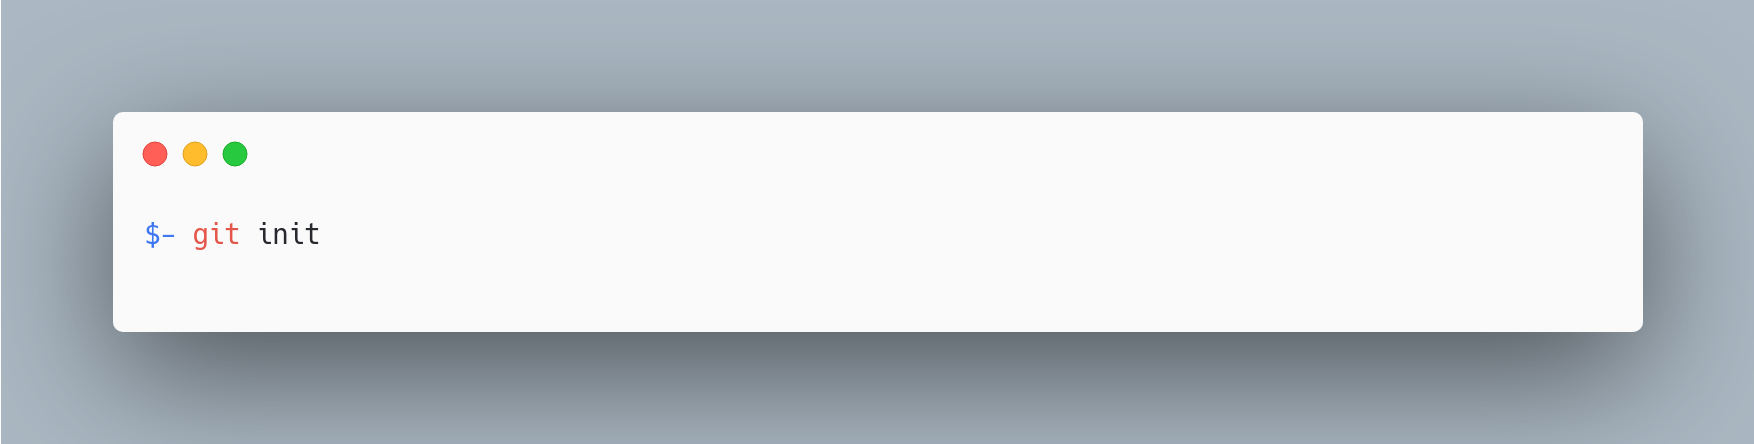
\includegraphics[width=1\textwidth]{./Imagenes/image35.png}
     \caption[Inicializar GIT]{Inicializar GIT}
         \end{figure}
    \newline
    \newline
    Creará una carpeta oculta (“/.git”) que nos permitirá manipular nuestro código con la línea de comandos de git, como crear ramas, hacer commit, hacer el merge de una rama etc.
    Para que esto funcione es necesario que el archivo creado anteriormente “package.json” conozca la ubicación remota de nuestro repositorio, se creó una cuenta en GITHUB  y se agregó un repositorio, el cual debemos copiar la dirección url y pegarla en el archivo “package.json”,  en el apartado llamado “repository” , en la llave “url” como se muestra en la imagen.
    Al la url que acabamos de copiar agregamos el prefijo “git+” y el postfijo “.git”.
    \newline
    \newline
     \begin{figure}[H]
    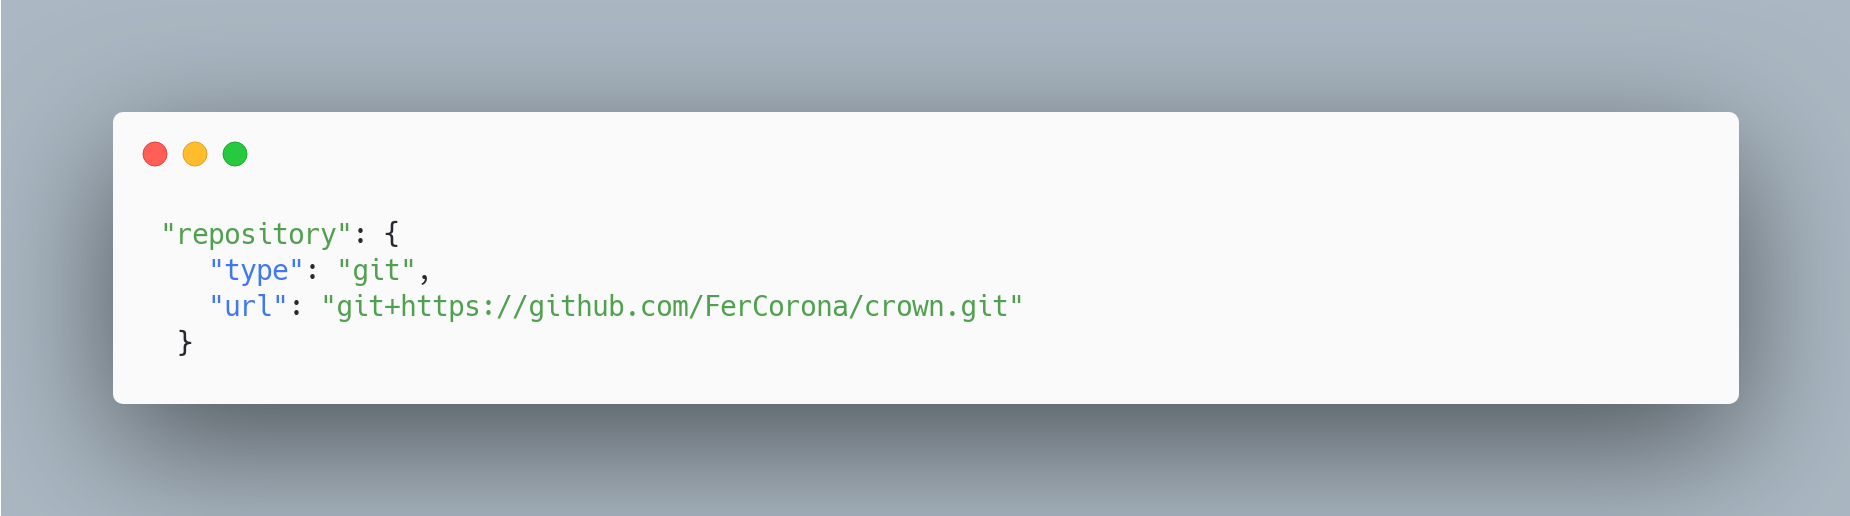
\includegraphics[width=1\textwidth]{./Imagenes/image4.png}
     \caption[Agregar repositorio existente]{Agregar repositorio existente}
         \end{figure}
    \newline
    \newline
    
    \subsection{Configuración Web-pack}
    Webpack es una tecnología utilizada en gran cantidad de proyectos de Front-end. Es útil cuando se trabaja en base a una estructura modular, en este caso modula nuestra librería para poder ser agregada en otros proyectos. Nos permite que el resultado final de nuestro proyecto sea menos pesado, esto es logrado por que concatena el código eliminando espacios no necesarios para el intérprete del navegador, lo que deja un archivo con código que no es del todo entendible para las personas pero que es muchos bits menos pesado para el navegador.
    También nos permite agregar cargadores para que pueda soportar SCSS, HTML JSX imágenes y otros archivos más.
    Para hacerlo funcionar debemos ejecutar una serie de comandos, que se enlistan a continuación, con ayuda de NPM.
    \newline
    \newline
     \begin{figure}[H]
    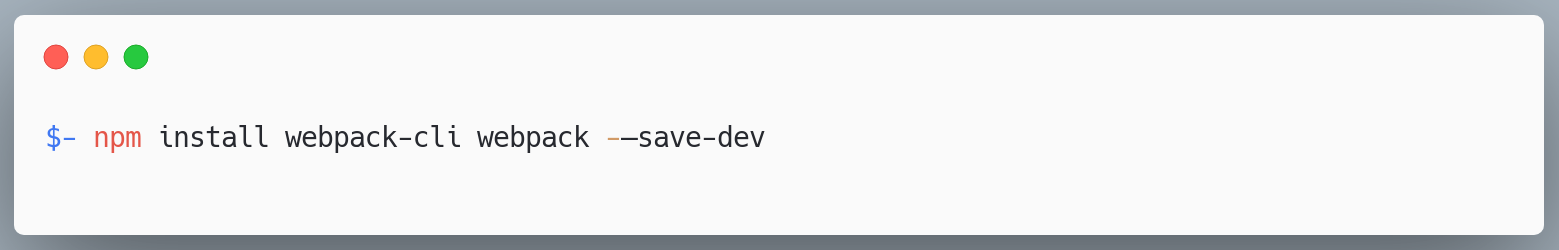
\includegraphics[width=1\textwidth]{./Imagenes/image3.png}
     \caption[Agregar Webpack]{Agregar Webpack}
         \end{figure}
    \newline
    \newline
    Los anteriores comandos agregan al proyecto en núcleo de Webpack, así como su cliente de comandos para la manipulación y visualización de archivos. Después de ejecutar los comandos se debe agregar los siguientes comandos en archivo “package.json”  en la sección de scripts, los script son los siguientes.
    \newline
    \newline
     \begin{figure}[H]
    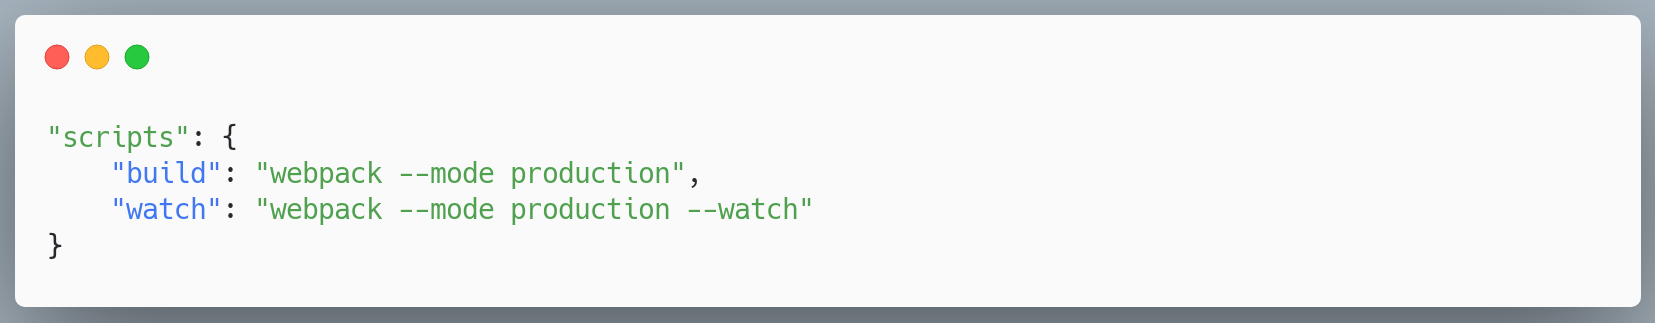
\includegraphics[width=1\textwidth]{./Imagenes/image6.png}
     \caption[Agregar scripts]{Agregar scripts}
         \end{figure}
    \newline
    \newline
    Los comandos agregados nos son de utilidad para:
    \begin{itemize}
    \item \textbf{Build:} Crear un archivo que estará listo para producción.
    \item \textbf{Watch:} Nos proporciona la misma funcionalidad que Build pero este, puede observar los cambios que estamos haciendo en tiempo real y actualizará el archivo final cada vez.
    \end{itemize}
    Para agregar configuración es necesario crear un archivo como se ilustra con el siguiente comando, estando en el directorio raíz de “crown”.
    \newline
    \newline
     \begin{figure}[H]
    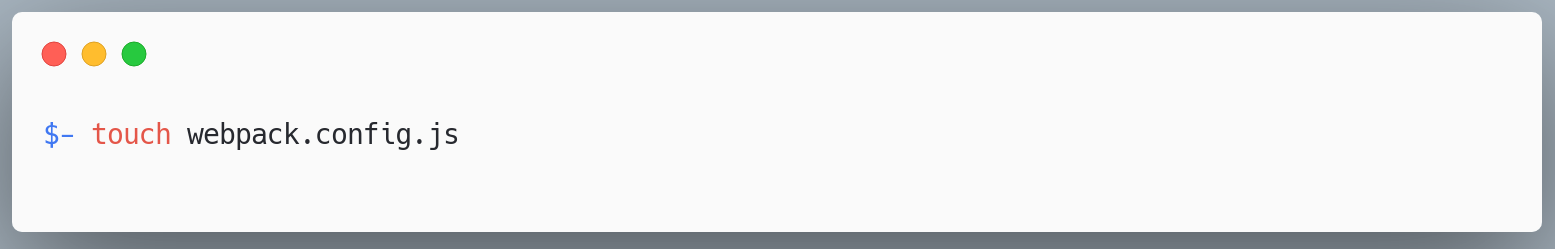
\includegraphics[width=1\textwidth]{./Imagenes/image38.png}
     \caption[Crear archivo vacío]{Crear archivo vacío}
         \end{figure}
    \newline
    Necesitamos agregar ciertos cargadores de Webpack para poder usar SASS y CSS, con el siguiente comando.
    \newline
    \newline
     \begin{figure}[H]
    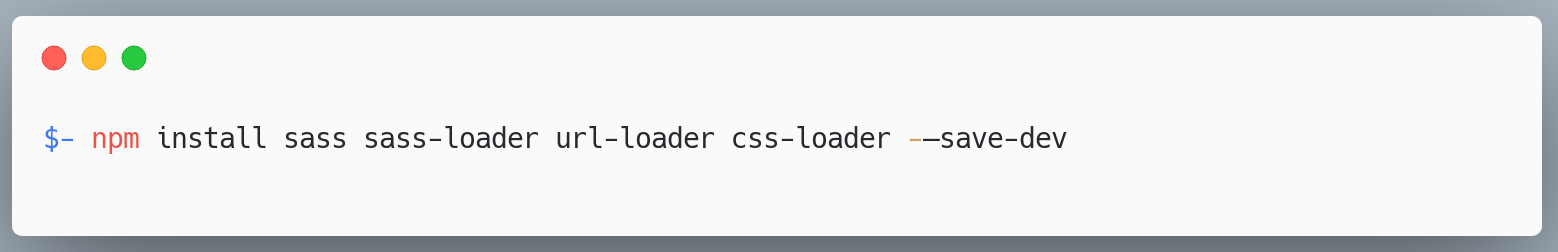
\includegraphics[width=1\textwidth]{./Imagenes/image8.png}
     \caption[Agregar cargadores de css]{Agregar cargadores de css}
         \end{figure}
    \newline
    \newline
    Con esto tenemos listas las dependencias necesarias para usar SASS / CSS y para poder manejar archivos como imágenes en JavaScript, tenemos que agregar la siguiente configuración en nuestro archivo Webpack.config.js.
    \newline
    \newline
     \begin{figure}[H]
    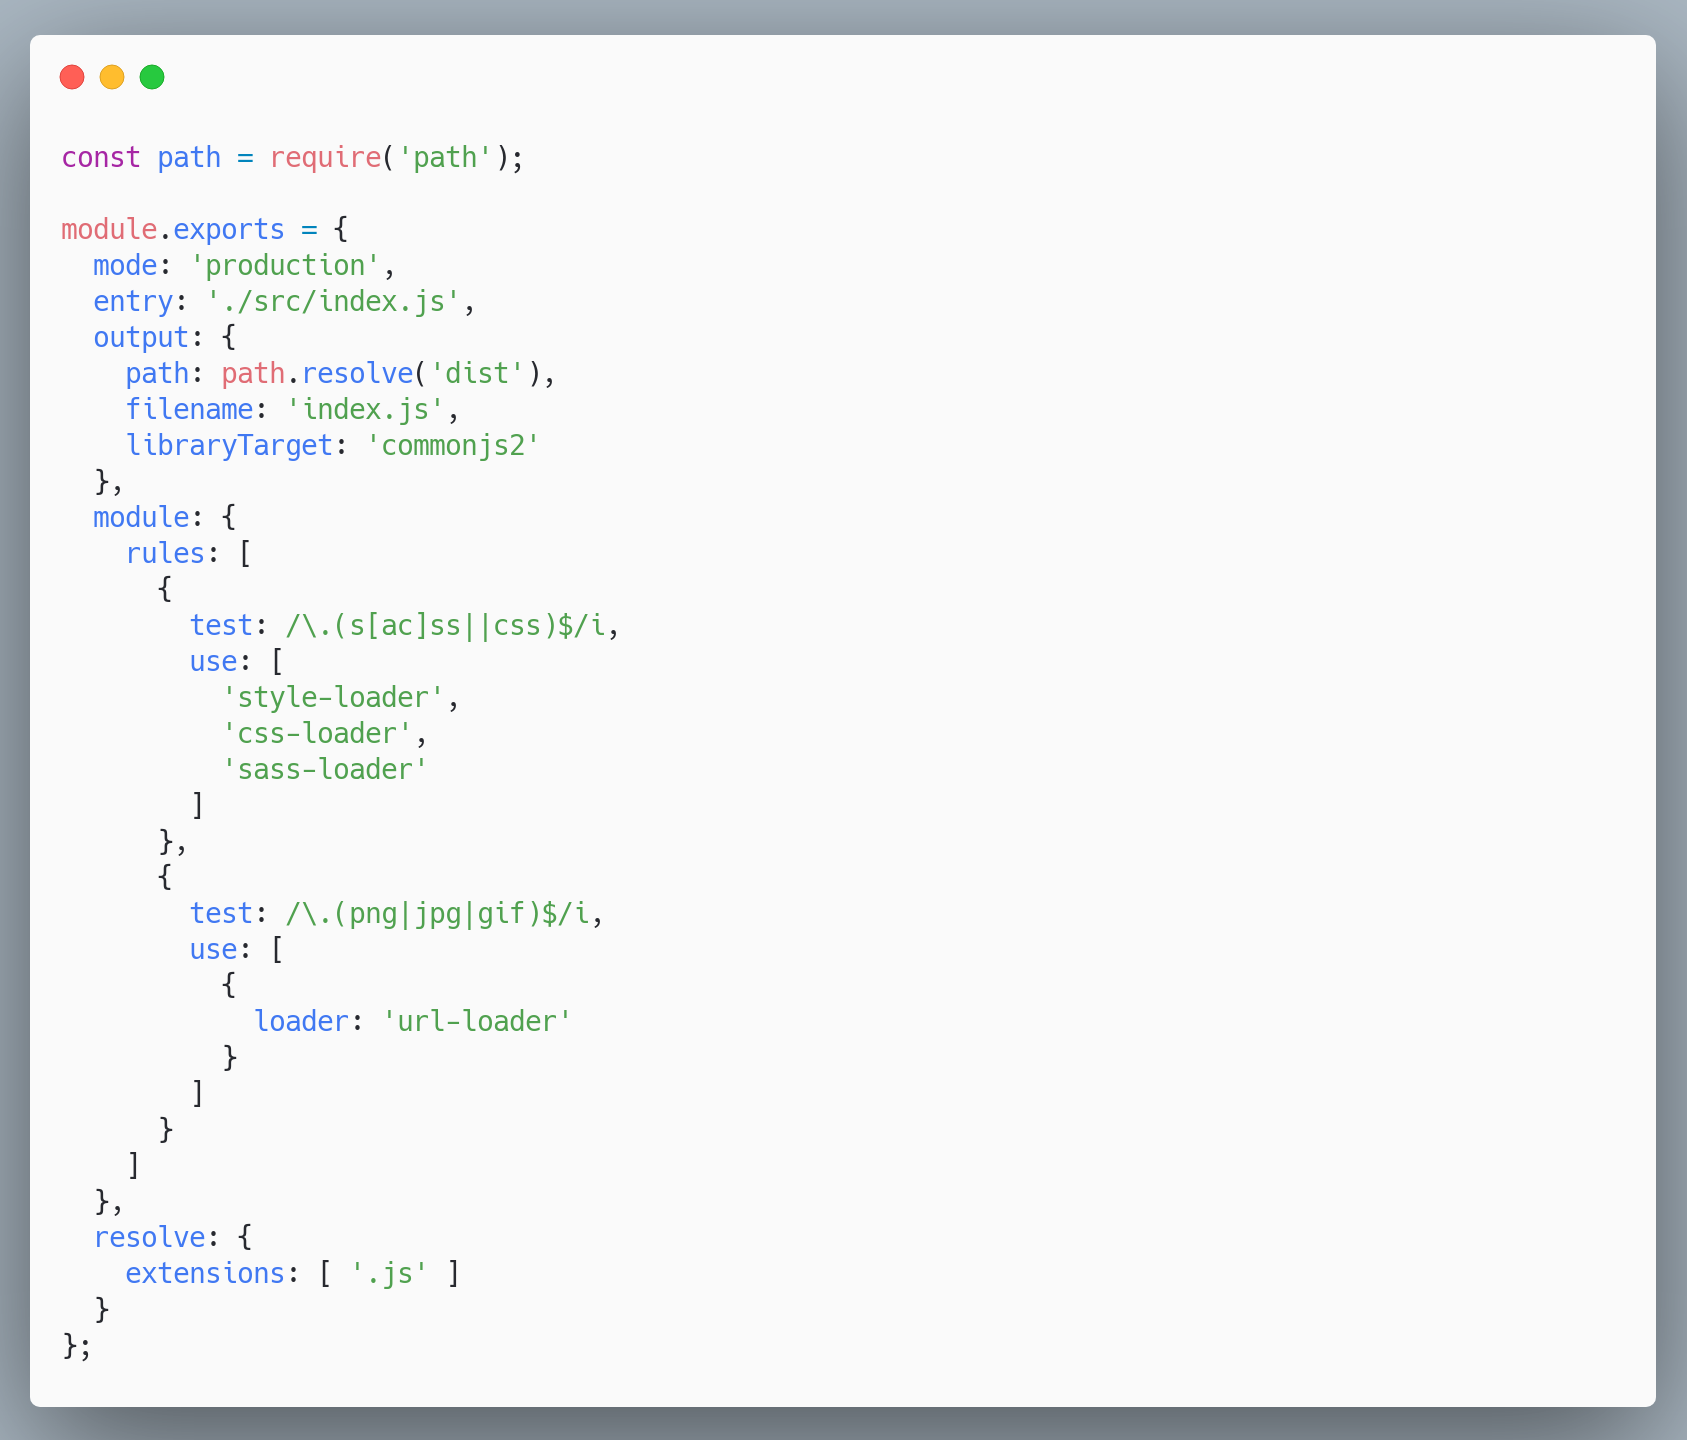
\includegraphics[width=1\textwidth]{./Imagenes/image2.png}
     \caption[Archivo final]{Archivo final}
         \end{figure}
    \newline
    La anterior configuración muestra cómo debe procesar cada tipo de archivo que encuentre dentro de nuestro proyecto, por eso dada una expresión regular que define extensiones de archivos puede usar un cargador a usar.
    Lo que es definido en la configuración es:
    \begin{itemize}
    \item \textbf{Entry: } Es el archivo inicial sobre el cual empezará el análisis del código si este tiene un import de otro archivo continuará sobre ese, esto generará un árbol. El directorio /src/index.js fue el dado para este caso.
    \item \textbf{Output: } Es el archivo en el que quedará la salida de nuestra librería en la dirección /dist/index.js
    \item \textbf{Rules: }Está incluido dentro de los módulos, esto agrega la manera en cómo se procesarán los archivos SCSS y CSS  con las dependencias style-loader, css-loader, sass-loader y por otra parte las imágenes con url-loader.
    \end{itemize}
    
    
    \subsection{Configuración Babel}
    Babel es un traductor de código JavaScript que permite convertir código de nuevas generaciones como el ES6 a versiones antiguas, extendiendo la compatibilidad a navegadores más viejos como Internet Explorer.
    Solo es necesario agregar las siguientes dependencias, con el siguiente comando.
    \newline
    \newline
     \begin{figure}[H]
    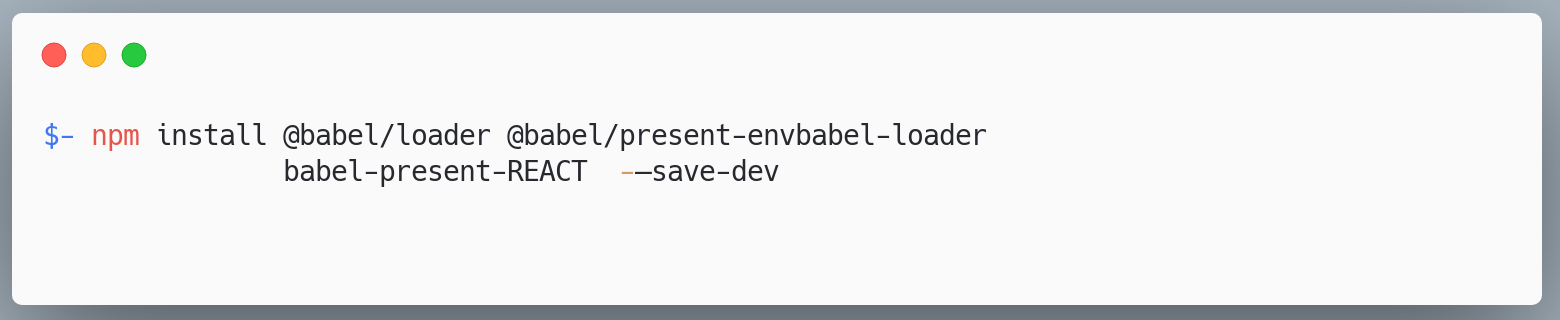
\includegraphics[width=1\textwidth]{./Imagenes/image36.png}
     \caption[Archivo Babel]{Archivo Babel}
         \end{figure}
    \newline
    \newline
    Después debemos crear un archivo en el directorio raíz llamado “.Babelrc”, al cual debemos agregar la siguiente configuración.
    \newline
    \newline
     \begin{figure}[H]
    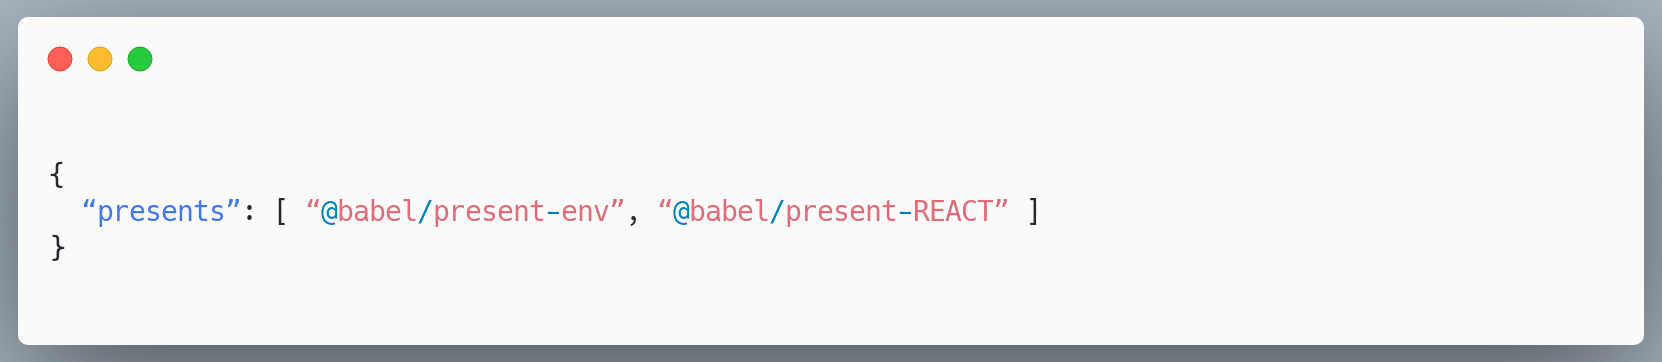
\includegraphics[width=1\textwidth]{./Imagenes/image17.png}
    \caption[Configurar Babel]{Configurar Babel}
    \end{figure}
    \newline
    \newline
    Y finalmente solo debemos agregar la siguiente configuración al archivo Webpack.config.js en el apartado de “rules” dentro de “module”.
    \newline
    \newline
     \begin{figure}[H]
    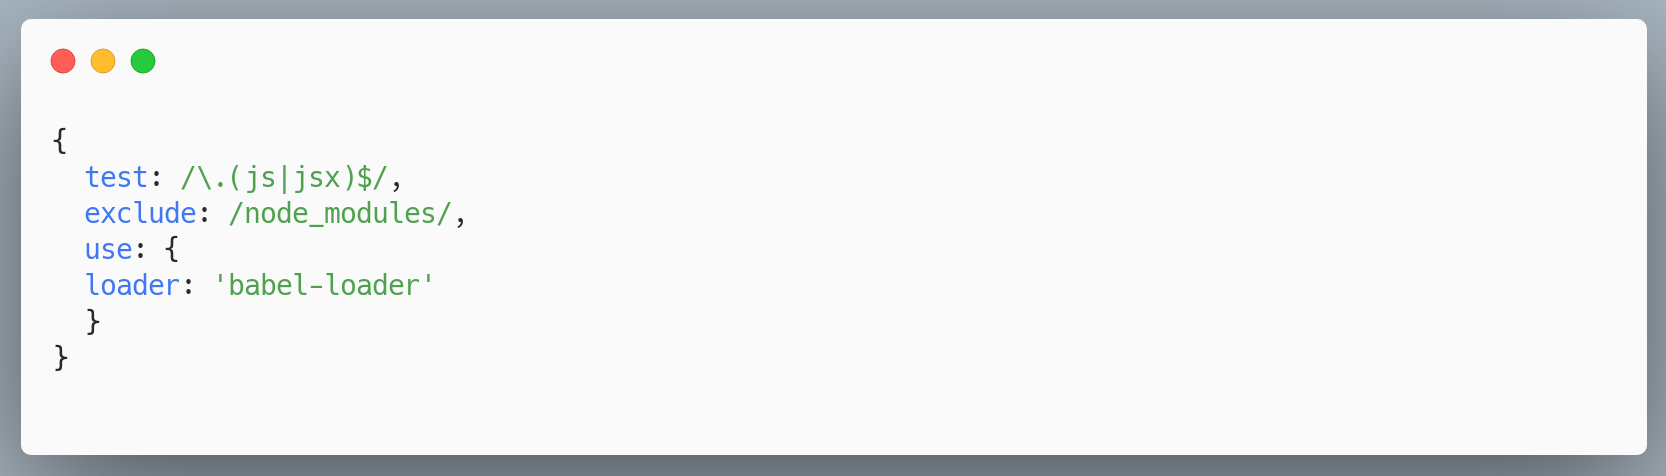
\includegraphics[width=1\textwidth]{./Imagenes/image1.png}
    \caption[Agregar Babel en Webpack]{Agregar Babel en Webpack}
    \end{figure}
    \newline
    \newline
    Esto para que WEWPACK sea el encargado de traducir el código con ayuda de Babel.
    
    
    \subsection{Agregar React Al Proyecto}
    React es una parte fundamental en el desarrollo de la presente librería y para agregarlo es necesario ejecutar el siguiente comando.
    \newline
    \newline
     \begin{figure}[H]
    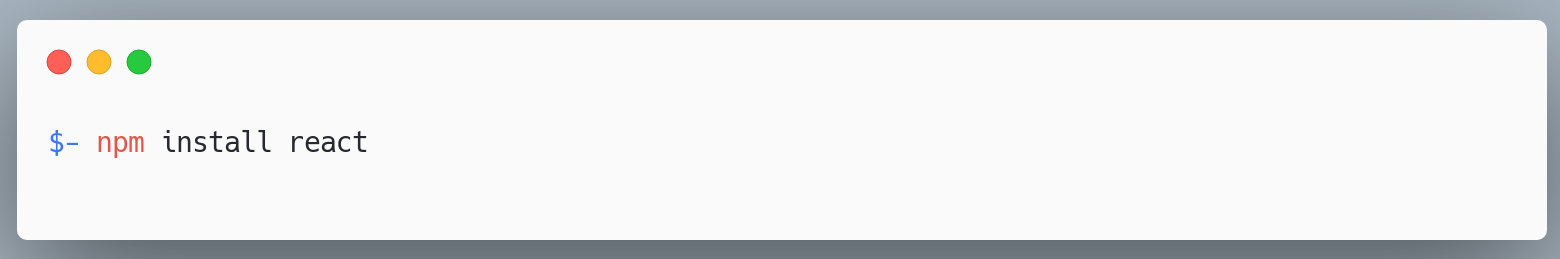
\includegraphics[width=1\textwidth]{./Imagenes/image23.png}
    \caption[Agregar React]{Agregar React}
    \end{figure}
    \newline
    \newline
    Para este comando no se agrega la bandera “–save-dev” al final, por que de esta manera forzamos a que cuando se instale esta librería también se instale React en caso de que no estuviera, ya que nuestra librería necesita React para su ejecución.
    
    
    \subsection{Configuración ESLint }
    Finalmente, para que nuestro espacio de desarrollo quede listo agregaremos ESLint que es un verificador de sintaxis, para tener un código limpio, con una clara indentación. Para que en toda la librería tengamos un código unificado. De igual manera no tendremos que preocuparnos por esto si no que al guardar el archivo obtenga el formato correcto.
    Para esto debemos ejecutar las siguientes dependencias en la terminal.
    \newline
    \newline
     \begin{figure}[H]
    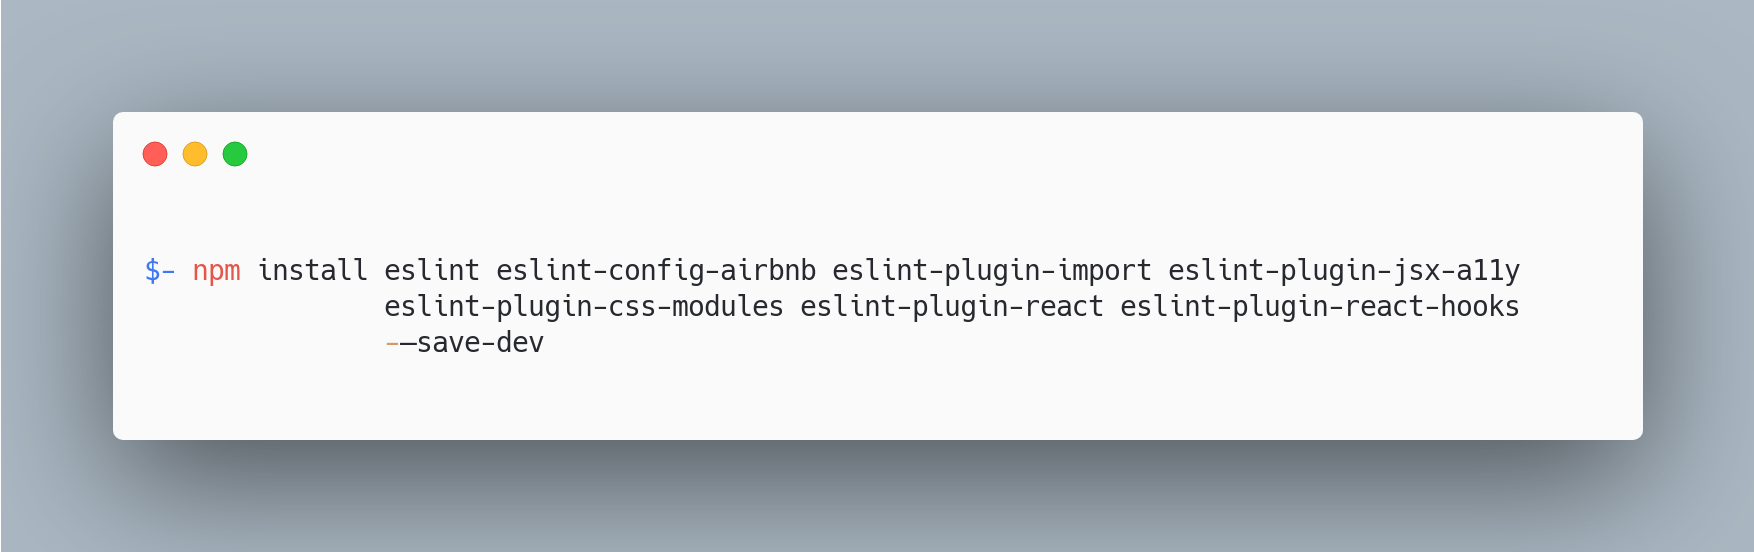
\includegraphics[width=1\textwidth]{./Imagenes/image14.png}
    \caption[Agregar ESLint]{Agregar ESLint}
    \end{figure}
    \newline
    \newline
    Dentro de las dependencias que agregamos se encuentran algunos complementos (plugins) que nos ayudan a dar formato a los archivos JSX, a verificar la sintaxis de React y  puede verificar que la importación de algún archivo realmente arroje un resultado.
    Debemos agregar un archivo en el que definiremos un conjunto de reglas específicas las cuales nuestros archivos van a cumplir, para agregar el archivo se debe ejecutar el siguiente comando.
    \newline
    \newline
     \begin{figure}[H]
    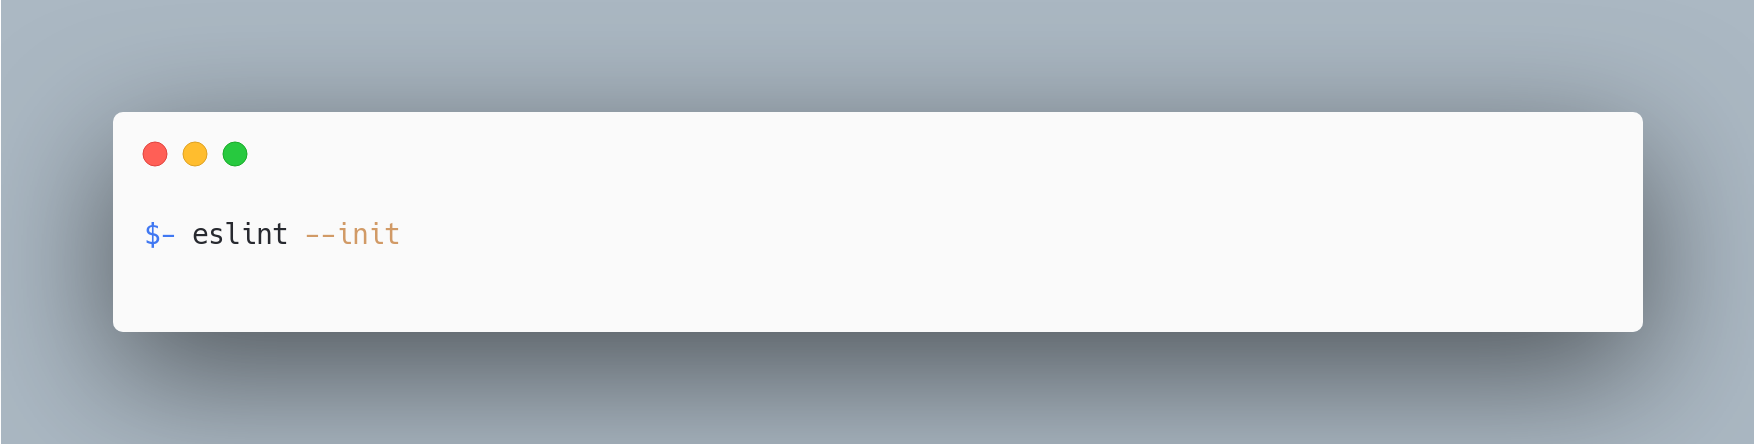
\includegraphics[width=1\textwidth]{./Imagenes/image32.png}
    \caption[Inicializar ESLint]{Inicializar ESLint}
    \end{figure}
    \newline
    \newline
    Después de ejecutar el comando este preguntara por datos para la configuración de ESLint, a continuación, se enlistan cada uno de los datos introducidos.
    \begin{itemize}
    \item \textbf{Uso de ESLint:  }Seleccionaremos el uso que le daremos a ESLint, que en este caso es checar sintaxis, encontrar problemas y forzar el estilo del código.
    \item \textbf{Tipo de módulos que usa el proyecto:} Seleccionaremos la opción JavaScript modules, por que es el tipo de importaciones y exportaciones que estaremos usando.
    \item \textbf{Framework por usar: }Seleccionaremos React.
    \item ¿Se usará TYPESCRIPT?: Se selecciona no. 
    \item ¿Donde se ejecutará?: Debemos seleccionar navegador.
    \item \textbf{Guía de estilos que se usará en el proyecto: } Nosotros elegiremos usar una guía popular  y después escogemos Airbnb.
    \item Formato del archivo de salida: Nosotros debemos escoger JavaScript.
    \end{itemize}
    Con esto tenemos todo listo para comenzar con el desarrollo de nuestra librería.
    \newpage

				
			\section {DESARROLLO}
				\subsection{Configuración Archivo Inicial}
El proyecto contendrá un nodo raíz el cual será el que tendrá los llamados al conjunto de elementos que tendrá nuestra librería. Anteriormente se creó un directorio llamado “src” en la raíz de “crown”, dentro de “src” debemos crear un archivo llamado “index.js” este es un archivo de JavaScript el cual definiremos como punto de inicio de Webpack  y a partir de este buscará todas las importaciones de otros submódulos. Con el siguiente comando creamos el archivo requerido.
\newline
\newline
     \begin{figure}[H]
    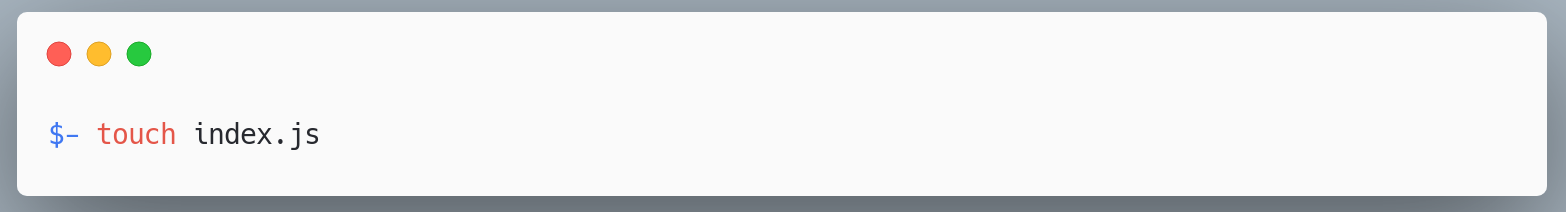
\includegraphics[width=1\textwidth]{./Imagenes/carbon.png}
    \caption[Inicializar archivo vacío]{Inicializar archivo vacío}
    \end{figure}
\newline
\newline
Dentro de este archivo debemos poner el llamado a cada elemento que se vaya agregando a nuestra librería ( Botones, Campos de texto, Tablas etc.), en la siguiente ilustración se muestra la manera en que se deben agregar los elementos.
\newline
\newline
\begin{figure}[H]
    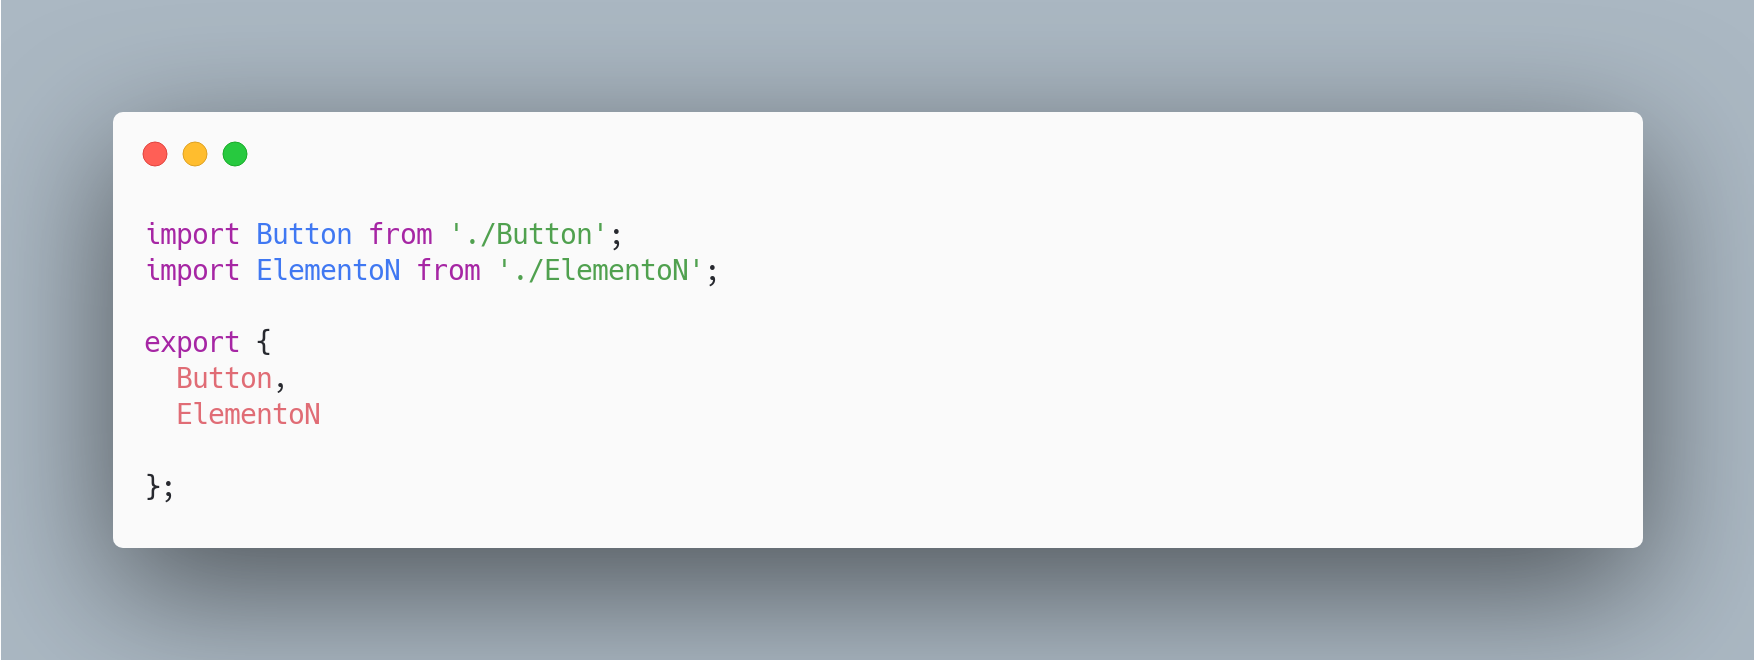
\includegraphics[width=1\textwidth]{./Imagenes/carbon-2.png}
    \caption[Inclusión de los elementos]{Inclusión de los elementos}
    \end{figure}
\newline
\newline
El primer bloque de código muestra la importación de cada uno de los elementos a nuestro archivo index, y la segunda parte exportamos un objeto de JAVASCRIPT con cada uno de los elementos.
Webpack analiza cada elemento que se incluye en el objeto y busca el contenido existente dentro de cada uno.
Cada uno de los elementos que se necesita agregar deben estar situados a la misma altura del archivo “index.js” esto dentro del directorio “src” para que puedan ser procesados.



\subsection{Elemento Botón}
El primer elemento que vamos a agregar es el botón, para esto creamos un directorio llamado “Botton” de la siguiente manera.
\newline
\newline
\begin{figure}[H]
    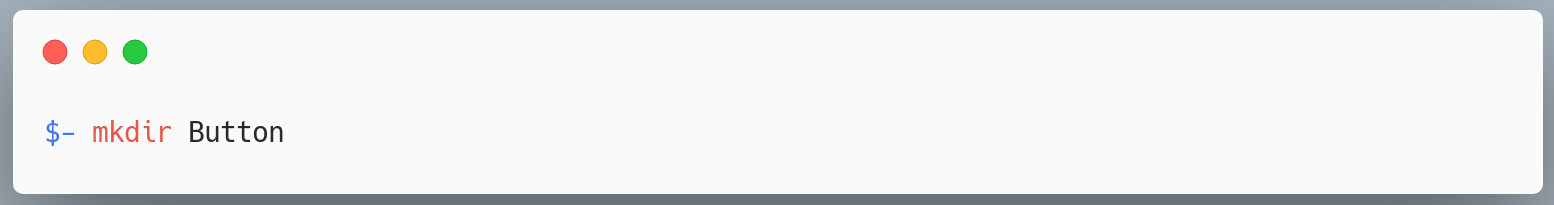
\includegraphics[width=1\textwidth]{./Imagenes/carbon-3.png}
    \caption[Crear directorio para el elemento Button]{Crear directorio para el elemento Button}
    \end{figure}
\newline
\newline
Y dentro de este directorio crearemos dos archivo que son los que incluirán el núcleo de nuestro botón, el primer archivo se llamará “index.js ” esto es así ya que por defecto, cuando importas un archivo que está dentro de un directorio, JAVASCRIPT toma el que es llamado “index.js” y no es necesario especificar este dato, esto lo podemos ver de manera clara en el archivo inicial “index.js” que está al mismo nivel que el directorio “Botton”, el cual importa el elemento Botton pero no especifica el archivo. Este archivo solamente hace el llamado al segundo archivo “Botton.js” que es el que tiene el código fuente del botón. 
\newline
\newline
\begin{figure}[H]
    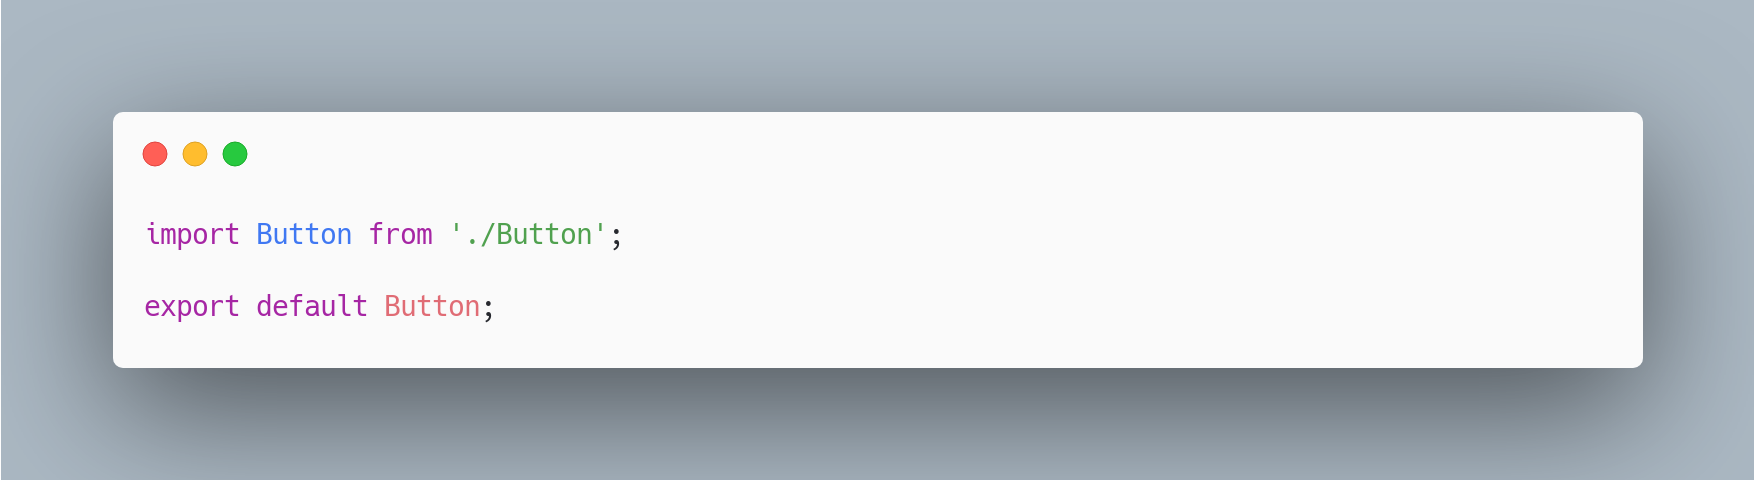
\includegraphics[width=1\textwidth]{./Imagenes/carbon-5.png}
    \caption[Contenido del elemento Button]{Contenido del elemento Button}
    \end{figure}
\newline
\newline
El segundo archivo ya mencionado “Botton.js”  hace el render de nuestro botón, y gestiona la configuración que el usuario final quiera asignarle.
En la siguiente tabla se muestran los props ( configuración inicial  ) del botón.
\newline
\newline
\begin{center}
 \begin{tabular}{ | c |  p{5cm}  | c | p{3cm} |} 
 \hline
 \textbf{Nombre} &  \textbf{Uso} &  \textbf{ Tipo de dato} &  \textbf{Valor por defecto}\\ [0.5ex] 
 \hline\hline
text & Texto que mostrará el botón.  &  Cadena de texto. & Click me! \\  [2.5ex] 
 \hline
onClick & Es la función que ejecutará cuando se hace click. & Funcion. & Función vacía. \\[2.5ex] 
 \hline
color &  Es el color del botón. & Cadena de texto. & --blue-4 \\[3.5ex] 
 \hline
 textColor & Es el color del texto en el botón. &  Cadena de texto. & --white \\[2.5ex] 
 \hline
borderColor & Es el color del borde del botón. & Cadena de texto. & --blue-4 \\ [2.5ex] 
 \hline
 type & Es el tipo de botón. & Cadena de texto. & Default \\ [2.5ex] 
 \hline
 shape & Es la forma del botón. Estos valores agregaran una curvatura, tenemos Round y SemiRound uno mas curvo que otro. & Cadena de texto. & Round \\ [2.5ex] 
 \hline
 shadow & Especifica si el botón debe tener una sombra. & Cadena de texto. & Booleano. \\ [2.5ex] 
 \hline
\end{tabular}
\end{center}
\newline
\newline
\newline
Los tipos (type) de botones que podemos tener son los siguientes.
\begin{itemize}
\item \textbf{Default:} Es el botón que se recomienda usar como principal.
\item \textbf{Secondary:} Es recomendable usarlo si ya se usa un botón default, para cuidar la jerarquía visual.
\item \textbf{Text:} Este es un botón sin contorno, debe ser usado para acciones con poca importancia.
\end{itemize}
Los colores que se usan son una constante definida por la librería ya que se considera que son cromáticamente compatibles entre ellos, este tema se abordará más adelante.
A continuación se muestra un fragmento del código que permite agregar la configuración requerida.
\newline
\newline
\begin{figure}[H]
    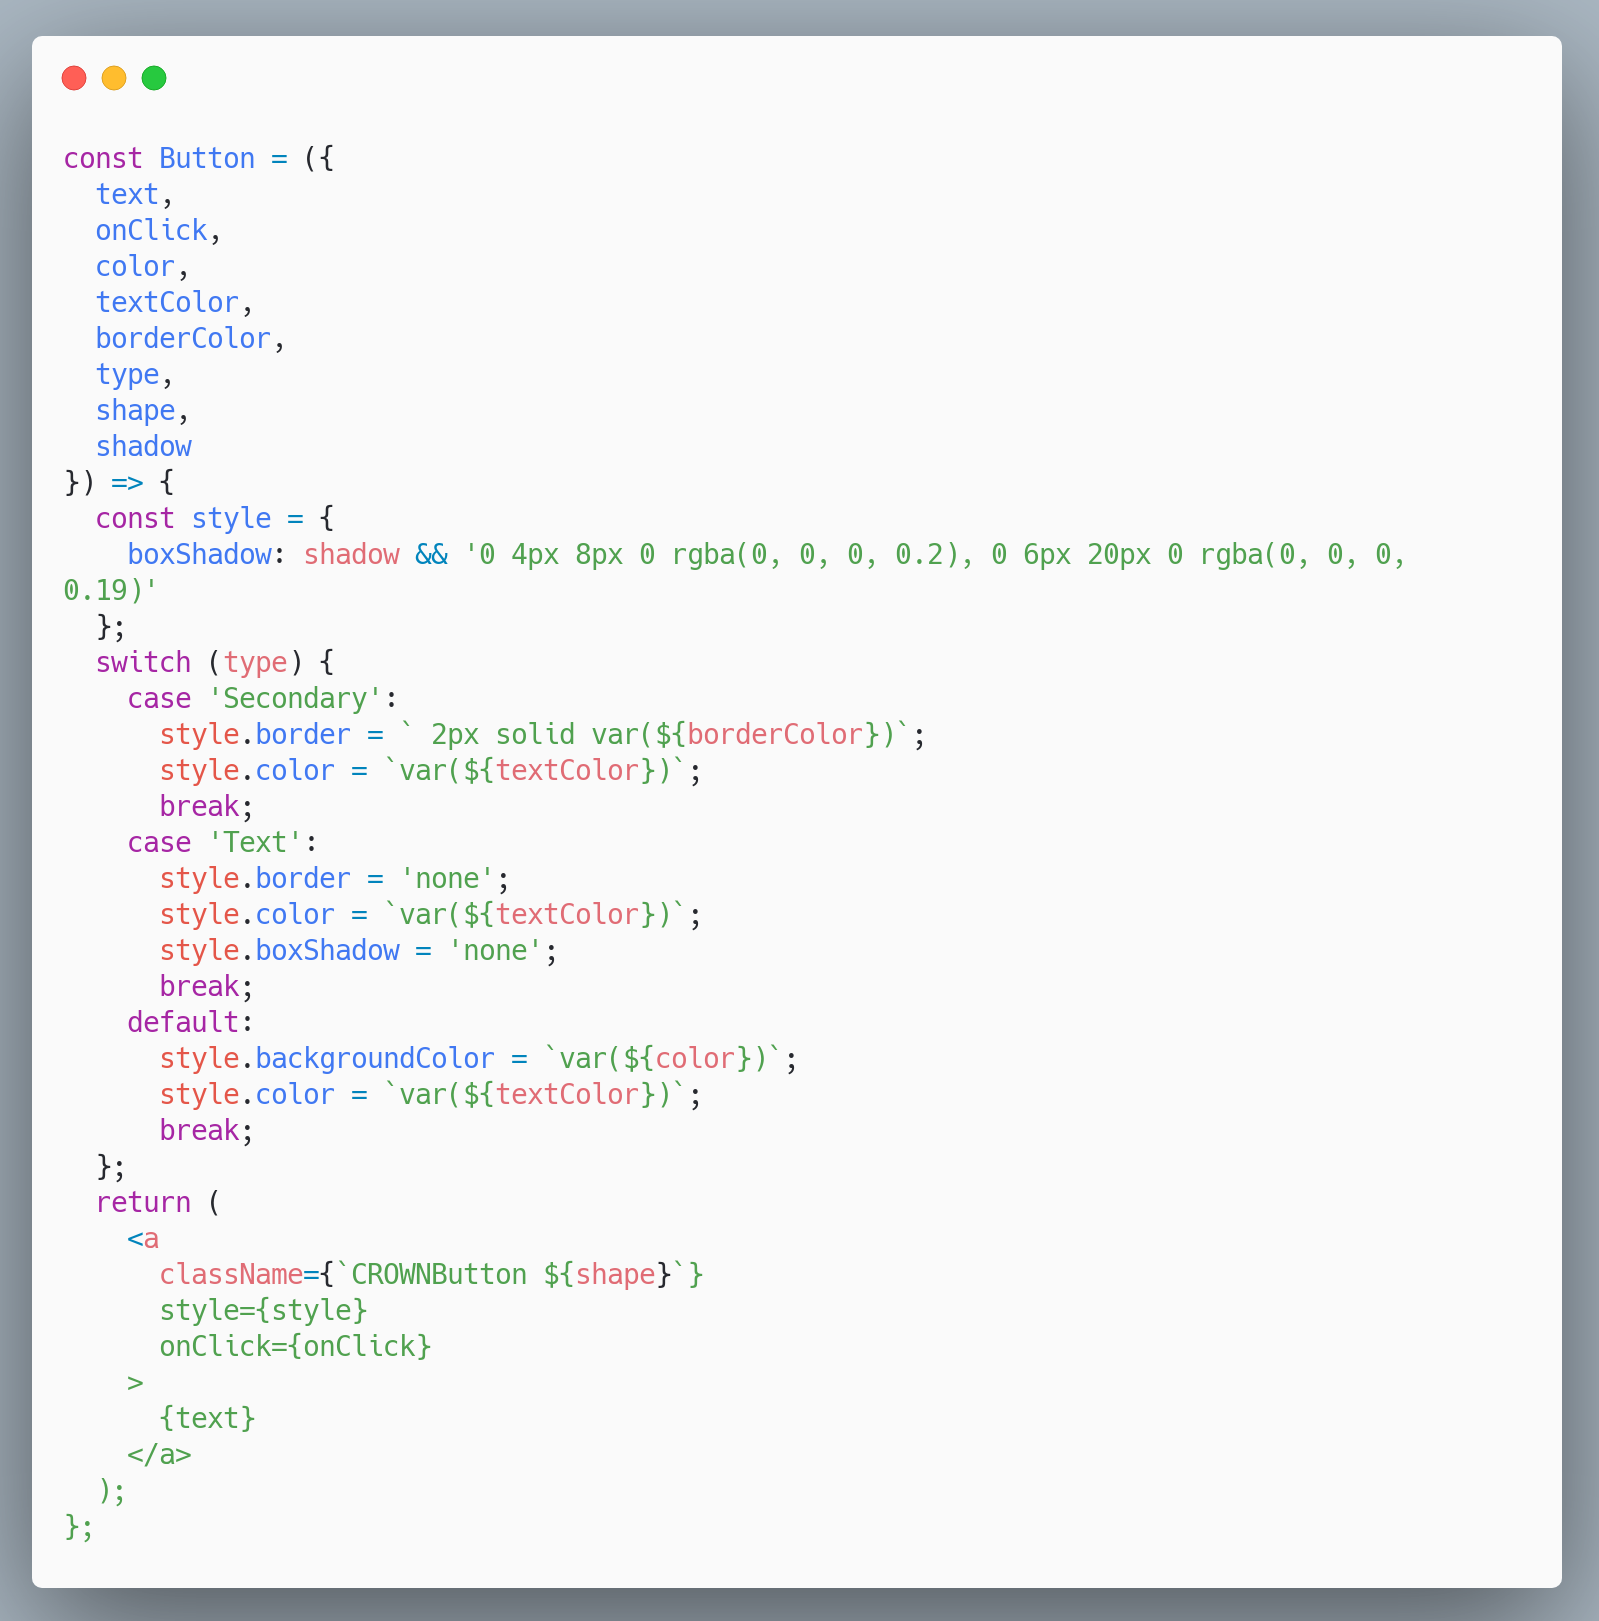
\includegraphics[width=1\textwidth]{./Imagenes/carbon-9.png}
    \caption[Código fuente del elemento Button]{Código fuente del elemento Button}
    \end{figure}
\newline
\newline
En la primera parte podemos ver una lista de la configuración dada,  después definimos un objeto llamado styles el cual agrega dentro de un switch el CSS para que sea mostrado de acuerdo al tipo ( type ) de botón que se quiere. Finalmente regresa HTML el cual es nuestro botón configurado.
Se puede observar que dentro de la etiqueta <a> tenemos “className” esto agrega la clase en la cual definiremos el CSS.
Dentro del archivo CSS agregamos el diseño base de nuestro botón, aquí tenemos el  tamaño de la letra, tamaño del botón, grosor de letra y otras cosas más.
\newline
\newline
\begin{figure}[H]
    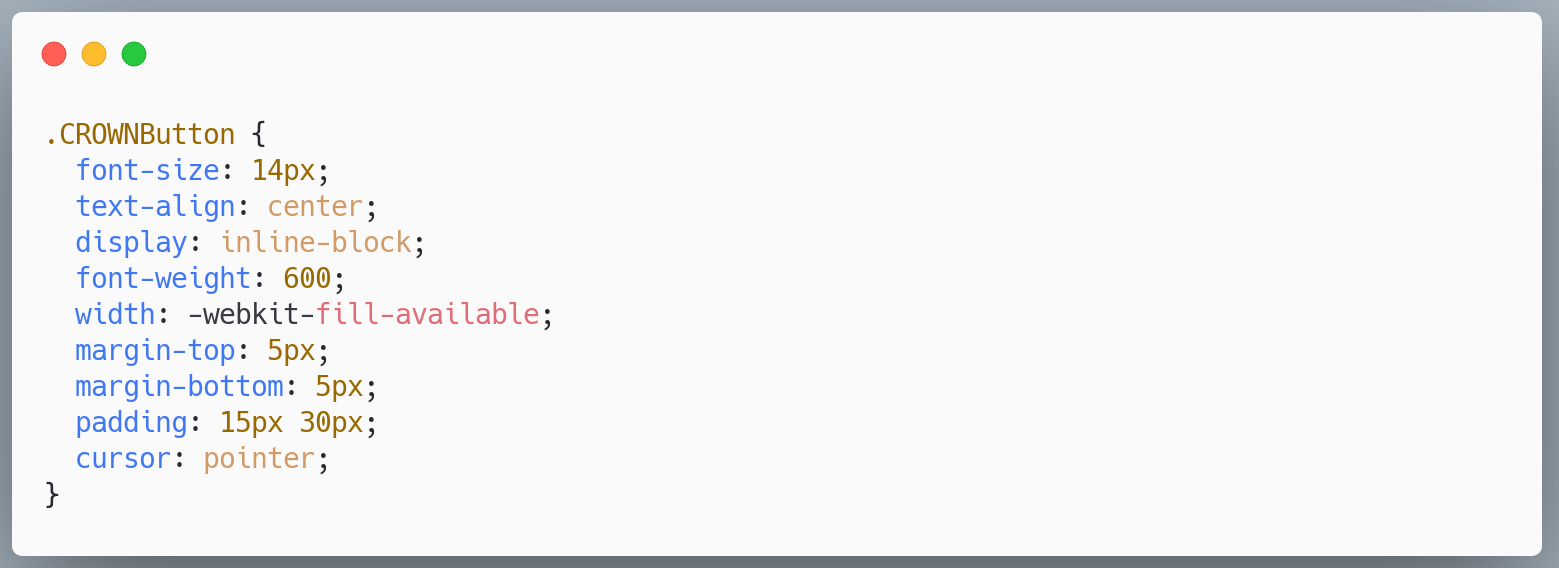
\includegraphics[width=1\textwidth]{./Imagenes/image26.png}
    \caption[Estilos del elemento Button]{Estilos del elemento Button}
    \end{figure}
\newline
\newline



\subsection{Elemento Label}
Ahora vamos a agregar el elemento Label que es un texto con el cual tenemos un formato estandarizado para tener un mejor diseño. En este elemento podemos dar parámetros de configuración como el tamaño, grosor y color que son los elementos básicos que se usan cuando estamos formateando con CSS nuestro texto. 
A continuación se presenta una lista de los parámetros y  su significado.
\newline
\begin{center}
 \begin{tabular}{ | c |  p{5cm}  | c | p{3cm} |} 
 \hline
 \textbf{Nombre} &  \textbf{Uso} &  \textbf{ Tipo de dato} &  \textbf{Valor por defecto}\\ [0.5ex] 
 \hline\hline
text 		& Este parámetro  indica el texto que vamos a mostrar.  &  Cadena de texto. 	& “I’m a label” \\  [2.5ex] 
 \hline
size 	        & Indicamos el tamaño del texto. Se cuenta con un conjunto de tamaños establecidos que se mencionan en el apartado de las constantes.       & Cadena de texto.  	& small \\[2.5ex] 
 \hline
color        & Es el color del texto.						    & Cadena de texto. 	& --black-0 \\[3.5ex] 
 \hline
 weight.   & Indicamos el grosor del texto. Se cuenta con un conjunto de tamaños establecidos que se mencionan en el apartado de las constantes.&  Cadena de texto. 	& regular \\[2.5ex] 
 \hline
\end{tabular}
\end{center}
\newline
\newline
Para el funcionamiento de la etiqueta de texto se tiene un componente de react en el cual se crea un objeto de JAVASCRIPT, se agrega la configuración del color, tamaño de texto y grosor. Finalmente se crea una etiqueta de HTML a la cual le damos nuestro objeto para que aplique el estilo y le ponemos el texto que se quiere mostrar.
\newline
\newline
\begin{figure}[H]
    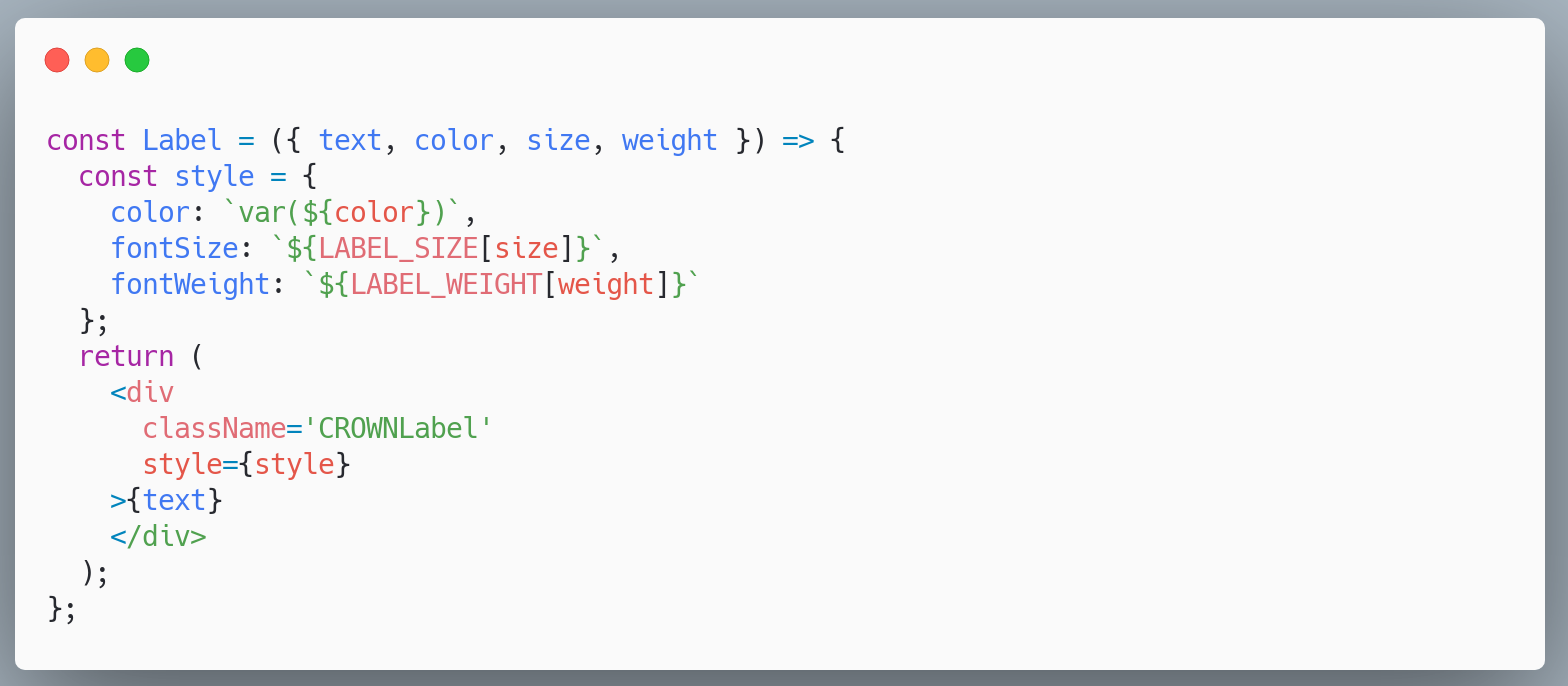
\includegraphics[width=1\textwidth]{./Imagenes/carbon-11.png}
    \caption[Código fuente del elemento Label]{Código fuente del elemento Label}
    \end{figure}
\newline
\newline



\subsection{Elemento Input Tex}
El input text es de utilidad para permitir la entrada de datos, y posteriormente puede ser procesado para enviarlos a algún servicio o procesarlos dentro de nuestra aplicación en donde es implementado.
Los datos de entrada que son necesarios para configurar el elemento se muestran a continuación.
\newline
\newline
\begin{center}
 \begin{tabular}{ | c |  p{5cm}  | c | p{3cm} |} 
 \hline
 \textbf{Nombre} &  \textbf{Uso} &  \textbf{ Tipo de dato} &  \textbf{Valor por defecto}\\ [0.5ex] 
 \hline\hline
placeholder &Es el texto que muestra el InputText si se desea poner.  &  Cadena de texto. 	& “Write on me!” \\  [2.5ex] 
 \hline
onChange & Es la función que va a hacer invocada cuando se escriba.     & Función vacía.  	& Función vacía.l \\[2.5ex] 
 \hline
nameState & Es el nombre con el cual se identifica en el estado.    & Cadena de texto.	& input \\[3.5ex] 
 \hline
 type   & Es la manera en como será interpretado por Input Text, estos son los que existen por defecto en HTML. Password etc.&  Cadena de texto.	& text \\[2.5ex] 
 \hline
 title  & Si se pone como “true” este agregara un Label antes del Input Text y no lo pondrá dentro.&  Booleano.	& false \\[2.5ex] 
 \hline
 extraStyle   & Si se desea agregar más estilos se puede poner el nombre de la clase CSS para poder ser manipulado.&  Cadena de texto. 	& Cadena vacía. \\[2.5ex] 
 \hline
\end{tabular}
\end{center}
\newline
\newline
La primera consideración que se tiene, es saber si se necesita tener un “Título” en nuestro Input Text, y si es así, se agrega un elemento Label antes,  para mostrar cual es el significado de nuestro label. Esto por ejemplo, si se quiere poner una entrada de texto para solicitar el correo electronico de cierta persona, esto puede estar dentro de el Input Texto denominado placeholder o afuera denominado title, por defecto title está desactivado y se activa enviando “true”.
Cuando se escribe sobre el campo de texto, este llama a la función “onChange” que recibe, se regresa el nombre de como está identificado en el estado de REACT y el valor que contiene el campo de texto.
Los demás parámetros de los estilos también son agregados en el siguiente código.
\newline
\newline
\begin{figure}[H]
    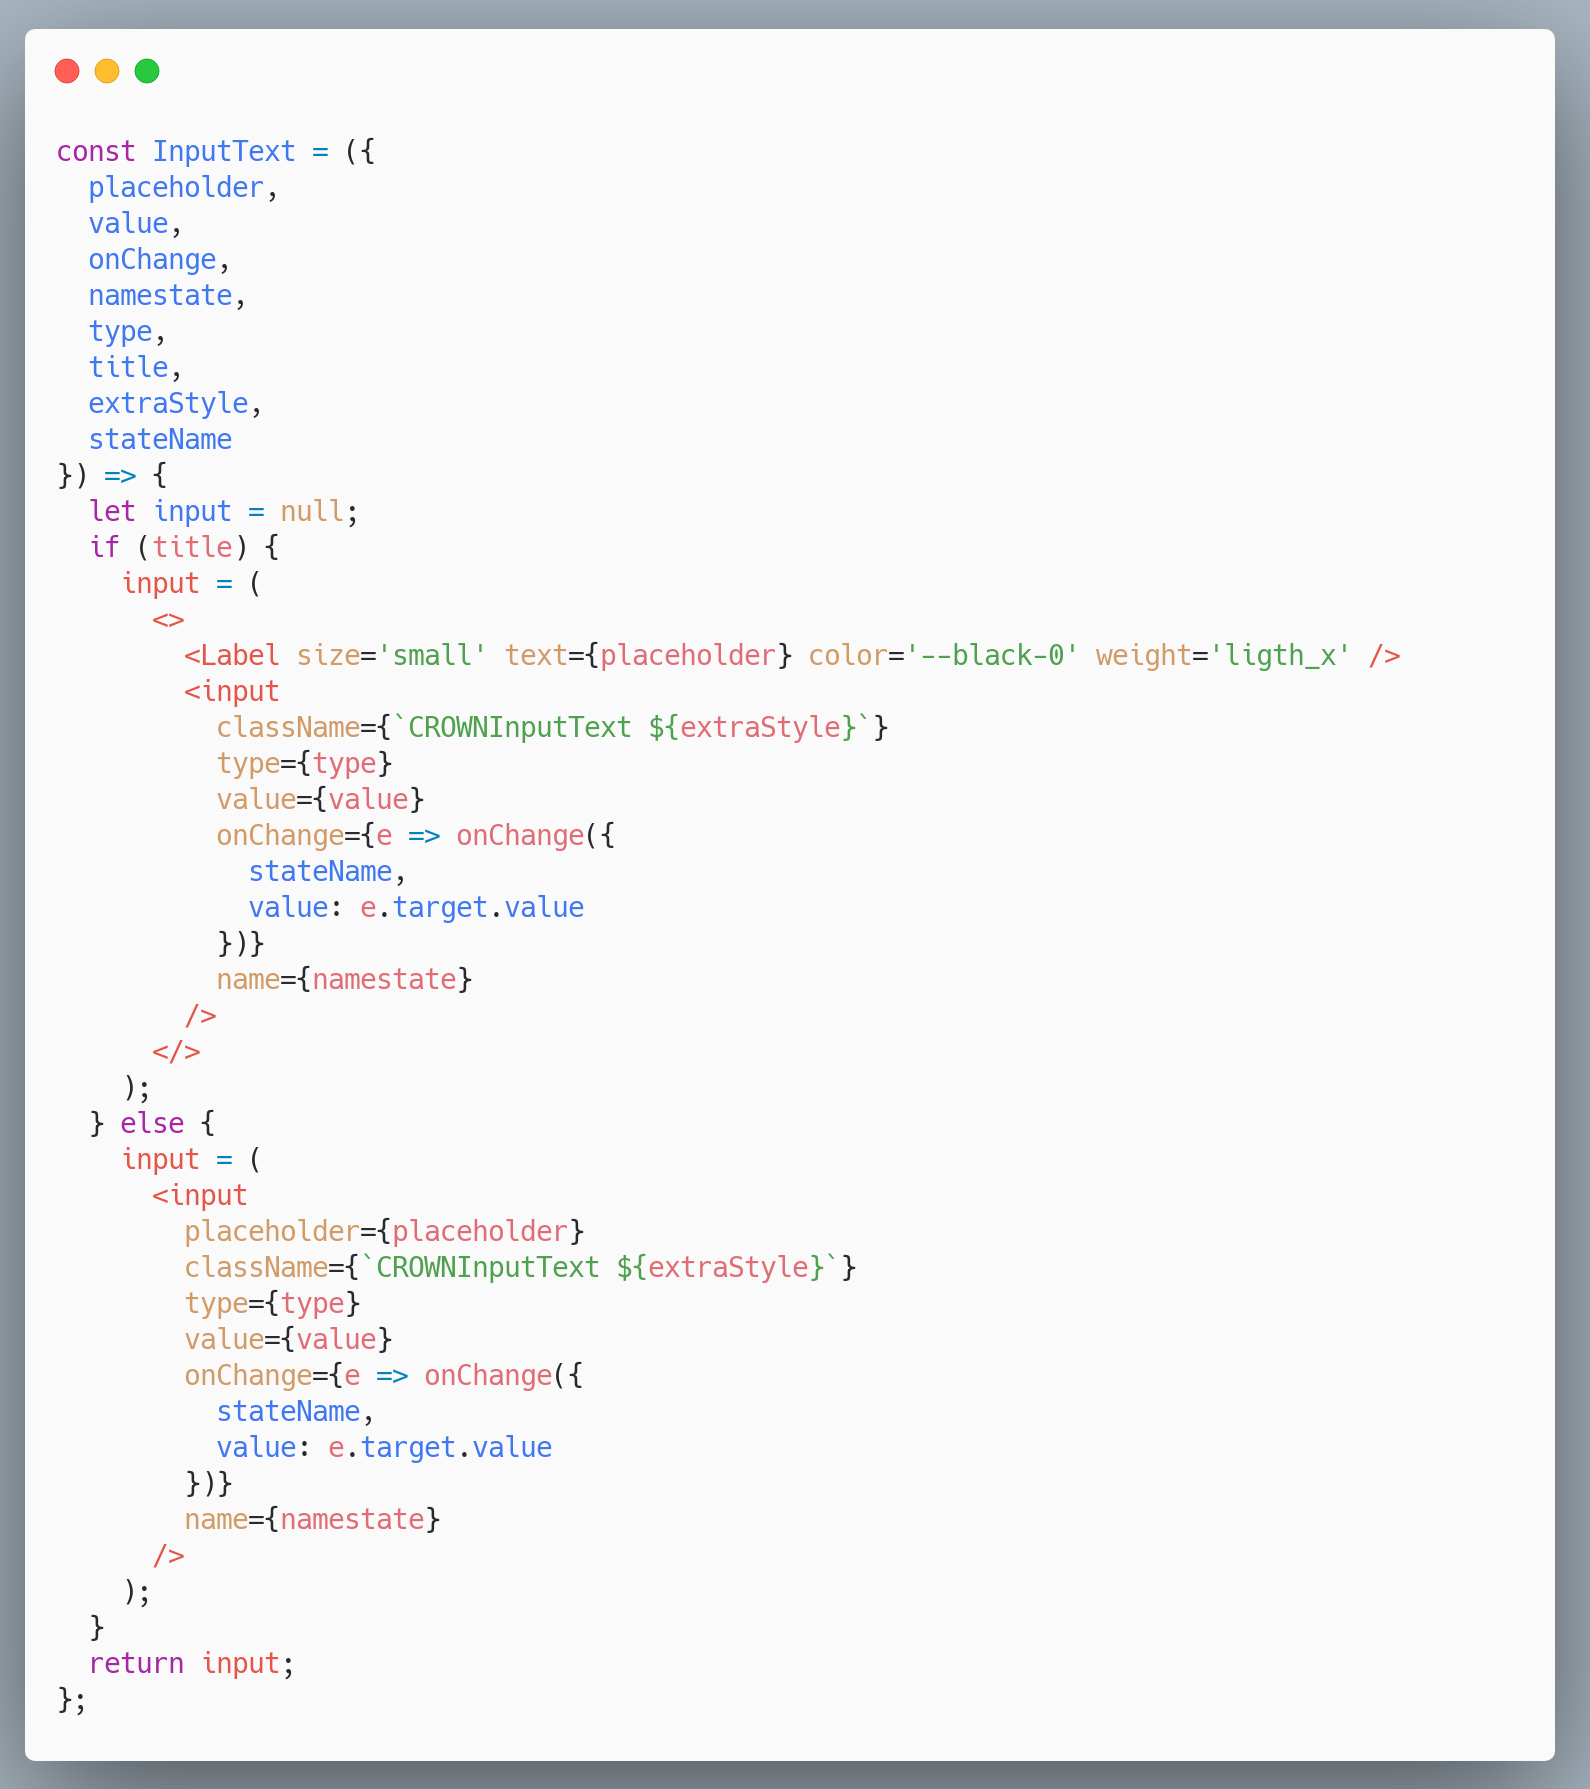
\includegraphics[width=1\textwidth]{./Imagenes/carbon-12.png}
    \caption[Código fuente del elemento InputText]{Código fuente del elemento InputText}
    \end{figure}
\newline
\newline



\subsection{Elemento Drop Down}
\subsection{Elemento Radio Button}
\subsection{Elemento Switch}
\subsection{Elemento Table}
\subsection{Elemento Check Box}
\subsection{Elemento Image}


				
			\section {TEST }
				Para garantizar el correcto funcionamiento de cada uno de los componentes se diseñan una serie de test para comprobar el comportamiento. Para esto se usará una librería llamada Jest \cite{jest} (Getting Started · Jest), para instalarla se debe ejecutar el siguiente comando.
\newline
\begin{figure}[H]
    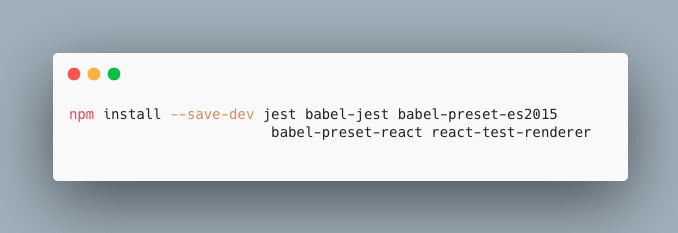
\includegraphics[width=1\textwidth]{./Imagenes/8.39t.png}
    \caption[Instalar dependencias]{Instalar dependencias}
    \end{figure}
\newline
Las dependencias instaladas con el comando anterior solo son usadas durante el desarrollo.

Dentro del directorio src debemos crear un subdirectorio llamado Test.
\newline
\begin{figure}[H]
    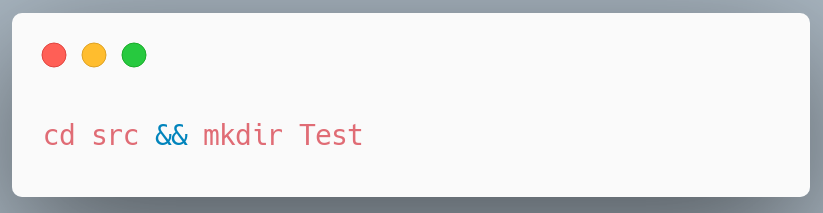
\includegraphics[width=1\textwidth]{./Imagenes/8.40t.png}
    \caption[Crear directorio]{Crear directorio}
    \end{figure}
\newline
Y dentro de este directorio crearemos un archivo por cada uno de los componentes llamado de la siguiente manera.
\begin{figure}[H]
   Nombre del Componente + . + test + . + js
    \centering
    \end{figure}
    
 Dentro de este se tendrán un código para asegurar el funcionamiento, por ejemplo para el componente Button se diseñó el siguiente test.
 \newline
\begin{figure}[H]biblioteca
    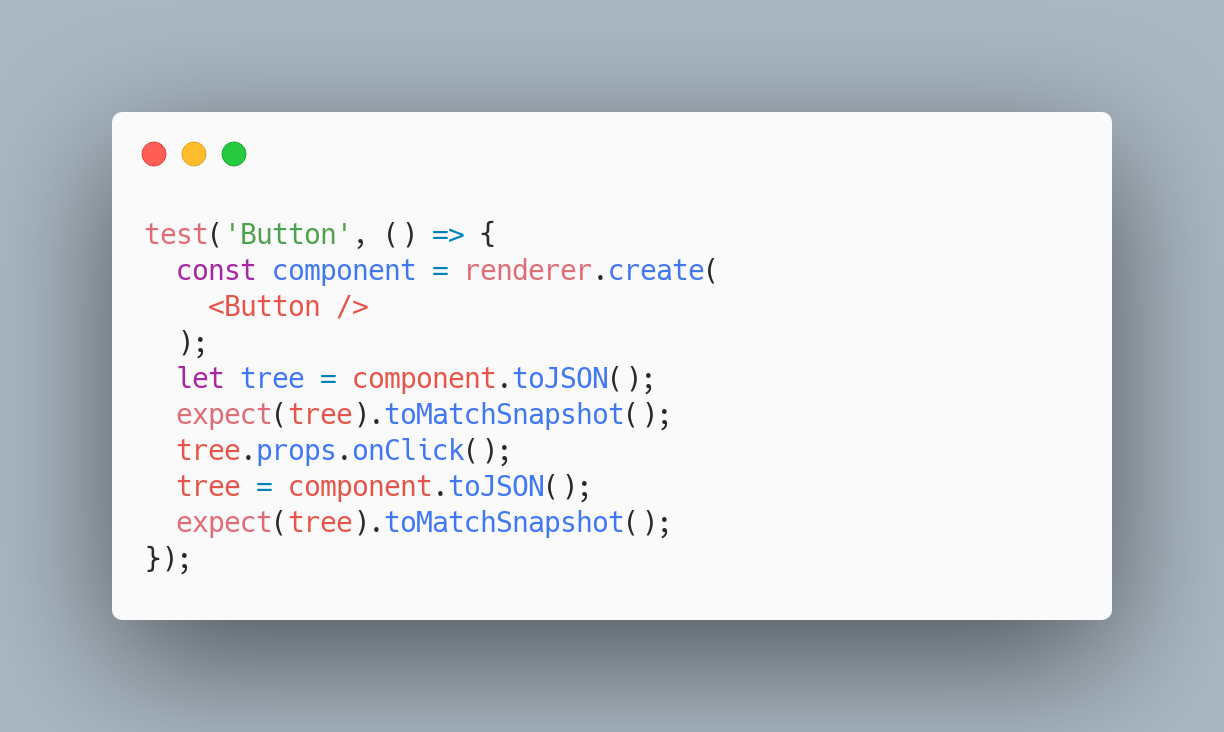
\includegraphics[width=1\textwidth]{./Imagenes/8.41t.png}
    \caption[Test del componente Button]{Test del componente Button}
    \end{figure}
\newline

El cual crea un componente, después crea una copia del resultado, y cada que se ejecute el test se debe comparar con la copia creada.
La segunda parte del test hacé click en el botón y verifica el funcionamiento.

Para poder ejecutar el todos los test, se debe agregar el siguiente comando en el archivo packeage.json.
 \newline
\begin{figure}[H]
    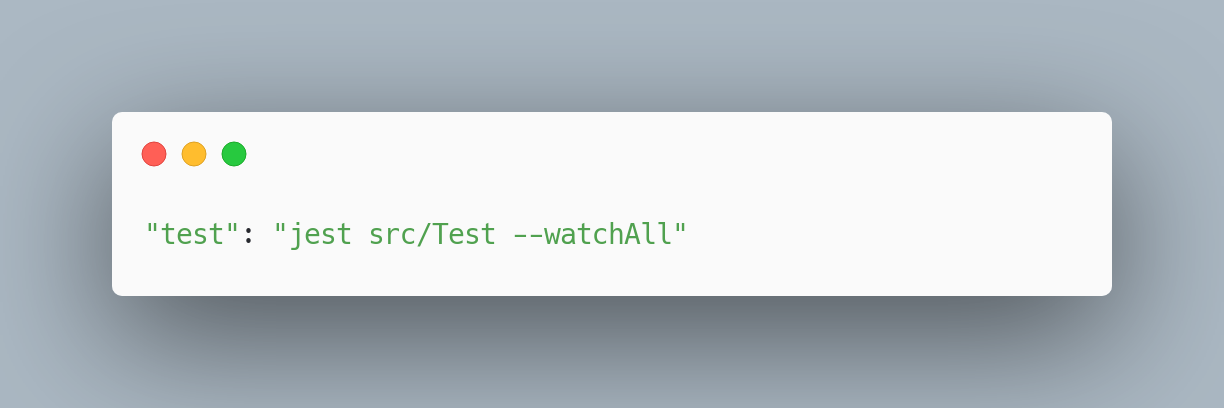
\includegraphics[width=1\textwidth]{./Imagenes/8.42t.png}
    \caption[Agregar comando]{Agregar comando}
    \end{figure}
\newline
\clearpage
			
		
		\chapter {RESULTADOS}
		
		\chapter {CONCLUSIONES Y RECOMENDACIONES}
		
		\chapter {FUENTES DE INFORMACIÓN}
		
		\chapter {ANEXOS}

\end{document}